%%%%%%%%%%%%%%%%%%%%%%%%%%%%%%%%%%%%%%%%%
% Masters/Doctoral Thesis 
% LaTeX Template
% Version 1.43 (17/5/14)
%
% This template has been downloaded from:
% http://www.LaTeXTemplates.com
%
% Original authors:
% Steven Gunn 
% http://users.ecs.soton.ac.uk/srg/softwaretools/document/templates/
% and
% Sunil Patel
% http://www.sunilpatel.co.uk/thesis-template/
%
% License:
% CC BY-NC-SA 3.0 (http://creativecommons.org/licenses/by-nc-sa/3.0/)
%
% Note:
% Make sure to edit document variables in the Thesis.cls file
%
%%%%%%%%%%%%%%%%%%%%%%%%%%%%%%%%%%%%%%%%%

%----------------------------------------------------------------------------------------
%	PACKAGES AND OTHER DOCUMENT CONFIGURATIONS
%----------------------------------------------------------------------------------------

\documentclass[11pt, oneside]{Thesis} % The default font size and one-sided printing (no margin offsets)

\graphicspath{{Pictures/}} % Specifies the directory where pictures are stored

\usepackage{epigraph}
\usepackage[square, numbers, comma, sort&compress]{natbib} % Use the natbib reference package - read up on this to edit the reference style; if you want text (e.g. Smith et al., 2012) for the in-text references (instead of numbers), remove 'numbers' 
\usepackage[font=small,format=plain,labelfont=bf,textfont=normal, justification=justified,singlelinecheck=false]{caption}
\hypersetup{urlcolor=blue, colorlinks=true} % Colors hyperlinks in blue - change to black if annoying
\title{\ttitle} % Defines the thesis title - don't touch this


\begin{document}

\frontmatter % Use roman page numbering style (i, ii, iii, iv...) for the pre-content pages

\setstretch{1.3} % Line spacing of 1.3

% Define the page headers using the FancyHdr package and set up for one-sided printing
\fancyhead{} % Clears all page headers and footers
\rhead{\thepage} % Sets the right side header to show the page number
\lhead{} % Clears the left side page header

\pagestyle{fancy} % Finally, use the "fancy" page style to implement the FancyHdr headers

\newcommand{\HRule}{\rule{\linewidth}{0.5mm}} % New command to make the lines in the title page
\newcommand{\uniname}{Universidad del Norte}

% PDF meta-data
\hypersetup{pdftitle={\ttitle}}
\hypersetup{pdfsubject=\subjectname}
\hypersetup{pdfauthor=\authornames}
\hypersetup{pdfkeywords=\keywordnames}

%----------------------------------------------------------------------------------------
%	TITLE PAGE
%----------------------------------------------------------------------------------------

\begin{titlepage}
\begin{center}

\textsc{\LARGE \uniname}\\[1.5cm] % University name
\textsc{\Large Master Thesis}\\[0.5cm] % Thesis type

\HRule \\[0.4cm] % Horizontal line
{\huge \bfseries Visual Object Tracking applying ensemble of multiple trackers}\\[0.4cm] % Thesis title
\HRule \\[1.5cm] % Horizontal line
 
\begin{minipage}{0.4\textwidth}
\begin{flushleft} \large
\emph{Author:}\\
Jorge Martinez Gomez % Author name - remove the \href bracket to remove the link
\end{flushleft}
\end{minipage}
\begin{minipage}{0.4\textwidth}
\begin{flushright} \large
\emph{Supervisor:} \\
\href{http://niebles.net}{Juan Carlos Niebles} % Supervisor name - remove the \href bracket to remove the link  
\end{flushright}
\end{minipage}\\[3cm]
 
\large \textit{A thesis submitted in fulfilment of the requirements\\ for the degree of Master of Science}\\[0.3cm] % University requirement text
\textit{in the}\\[0.4cm]
Computer Vision Research Group\\Electrical and Electronics engineering department\\[2cm] % Research group name and department name
 
{\large \today}\\[4cm] % Date
%\includegraphics{Logo} % University/department logo - uncomment to place it
 
\vfill
\end{center}

\end{titlepage}


\clearpage % Start a new page

%----------------------------------------------------------------------------------------
%	QUOTATION PAGE
%----------------------------------------------------------------------------------------

\pagestyle{empty} % No headers or footers for the following pages

\null\vfill % Add some space to move the quote down the page a bit

\textit{``Thanks to my solid academic training, today I can write hundreds of words on virtually any topic without possessing a shred of information, which is how I got a good job in journalism."}

\begin{flushright}
Dave Barry
\end{flushright}

\vfill\vfill\vfill\vfill\vfill\vfill\null % Add some space at the bottom to position the quote just right

\clearpage % Start a new page

%----------------------------------------------------------------------------------------
%	ABSTRACT PAGE
%----------------------------------------------------------------------------------------

\addtotoc{Abstract} % Add the "Abstract" page entry to the Contents

\abstract{\addtocontents{toc}{\vspace{1em}} % Add a gap in the Contents, for aesthetics

The Thesis Abstract is written here (and usually kept to just this page). The page is kept centered vertically so can expand into the blank space above the title too\ldots
}

\clearpage % Start a new page

%----------------------------------------------------------------------------------------
%	ACKNOWLEDGEMENTS
%----------------------------------------------------------------------------------------

\setstretch{1.3} % Reset the line-spacing to 1.3 for body text (if it has changed)

\acknowledgements{\addtocontents{toc}{\vspace{1em}} % Add a gap in the Contents, for aesthetics
%\epigraph{Not enough people in this world, I think, carry a cosmic perspective with them. It could be life-changing.}{Neil deGrasse Tyson}
%\epigraph{TheBigBangTheory: When geeky scientists can be main characters in a hit primetime series, you know there's hope for the world.}{Neil deGrasse Tyson}

\epigraph{Not enough people do things that leave others to wonder.  RT @BrianMendicino: Wondering why @neiltyson is watching Glee.}{Neil deGrasse Tyson}

The acknowledgements and the people to thank go here, don't forget to include your project advisor\ldots
}
\clearpage % Start a new page

%----------------------------------------------------------------------------------------
%	LIST OF CONTENTS/FIGURES/TABLES PAGES
%----------------------------------------------------------------------------------------

\pagestyle{fancy} % The page style headers have been "empty" all this time, now use the "fancy" headers as defined before to bring them back

\lhead{\emph{Contents}} % Set the left side page header to "Contents"
\tableofcontents % Write out the Table of Contents

\lhead{\emph{List of Figures}} % Set the left side page header to "List of Figures"
\listoffigures % Write out the List of Figures

\lhead{\emph{List of Tables}} % Set the left side page header to "List of Tables"
\listoftables % Write out the List of Tables

%----------------------------------------------------------------------------------------
%	DEDICATION
%----------------------------------------------------------------------------------------

\setstretch{1.3} % Return the line spacing back to 1.3

\pagestyle{empty} % Page style needs to be empty for this page

\dedicatory{For/Dedicated to/To my\ldots} % Dedication text

\addtocontents{toc}{\vspace{2em}} % Add a gap in the Contents, for aesthetics

%----------------------------------------------------------------------------------------
%	THESIS CONTENT - CHAPTERS
%----------------------------------------------------------------------------------------

\mainmatter % Begin numeric (1,2,3...) page numbering

\pagestyle{fancy} % Return the page headers back to the "fancy" style

% Include the chapters of the thesis as separate files from the Chapters folder
% Uncomment the lines as you write the chapters


\input{Chapters/introduction}
% Chapter Template

\chapter{Moving Object Detection Approaches, Challenges, Datasets and Object Tracking} % Main chapter title

\label{chapter2} % Change X to a consecutive number; for referencing this chapter elsewhere, use \ref{ChapterX}

\lhead{Chapter 2. \emph{Moving Object Detection Approaches, Challenges and Object Tracking}} 

An object can be considered simply as nothing but an entity of interest used for further analysis. These elements can be represented by their shape \textbf{Cite here} or appearance \textbf{cite color histograms, etc.}. In order to track objects, selecting the right features plays a critical role. In general, the most important property of a visual feature is its uniqueness so that could be easily distinguished from other objects. Mostly features are chosen manually by the user depending on the application domain. this problem of automatic feature selection has receibed significant attention in the pattern recognition community. The most common visual features selections are color, edges, displacement vectors and textures.

Among all features, color is the one of the most widely used feature for tracking. However, color features are sensity to illumination variation. To tackle this problem, in scenarios where this effect is inevitable, other features are incorporated to model object appearance.

\section{Moving Object Detection}

In a video, there are two sources of information that can be used for object detection and tracking: Visual features (color, texture and shape) and motion information. Robust approaches suggest that combining the statistical analysis of visual features and temporal analysis of motion information. Moving object detection targets the extraction of moving objects that are of interest in sequences (e.g. people and vehicles).

A large number of methodologies have been proposed for object tracking, focusing on the task of object detection first. Most of them apply combinations and intersections among different methodologies, making it very difficult to create a uniform classification of existing approaches. This section classifies different approaches available for object detection from videos.

\subsection{Background Substraction}

Background subtraction is a commonly used technique for object segmentation in static scenarios \cite{McIvor2000}. This task consist in detecting moving regions by subtracting the current image pixel-by-pixel from a reference background image. The pixels above some threshold are classified as foreground (belongs to an object). The background image is created averaging images over time in an intiialization period, and is updated with new images to adapt to dynamic scene changes. Also, the foreground map is followed by morphological operations such as closing and erosion (elimination of small-sized blobs).

Although background subtraction techniques extracts well most of the relevant pixels, this method is sensitive to changes when some background and foreground pixels have similar value.

\begin{figure}[h!]
	\centering
		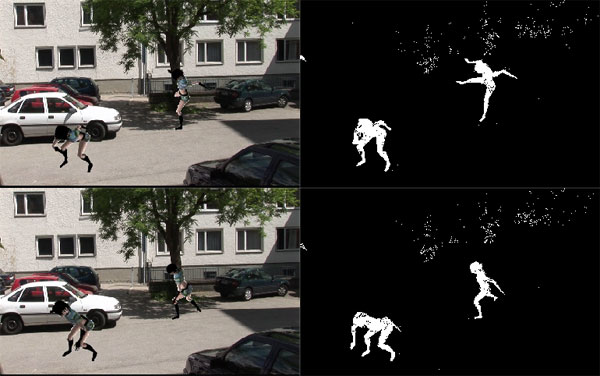
\includegraphics[width=0.7\linewidth]{Figures/bg_sub.jpg}
	\caption{Object detection using Gaussian Mixture Models for background subtraction \cite{Pham2010}. foreground pixels are drawn in white.}
	\label{fig::bg_sub}
\end{figure}

\subsection{Temporal differencing}

In temporal differencing, objects are detected by taking pixel-by-pixel difference of consecutive frames (generally two or three) in a video sequence. This method is most common for moving object detection in scenarios where camera is moving. Unlike static camera scenarios, the background is changing in time for moving camera (not appropiate to create a background model). Alternatively, the moving object is detected by taking the difference between frames $t - 1$ and $t$.

This method is highly adaptive to dynamic changes in the scene as most recent frames are involved in the process. However, it fails detecting small regions as moving objects (ghost regions). Detection will not be correct also, for objects that preserve uniform regions (static objects).

A two-frame differencing method is presented in \cite{Lipton1998a}, where the pixels that satisfy the following equation are marked as foreground.\\
\centerline{$|I_t(x,y), I_{t-1}(x,y)|>Th$}

Other methods were developed in order to overcome drastic changes of two frame differencing in some cases. For instance, a three-frame differencing method \cite{Wang2003} and a hybrid method that combines three-frame differencing with an adaptive background subtraction model \cite{Collins2000}.

\subsection{Statistical Approaches}

Statistical characteristics of pixels have been used, in order to overcome shortcomings between frames of basic background subtraction methods. The approaches consist in keeping and updating pixels statistics that belong to the background model. Foreground pixels are identified by comparing each pixel's statistics with that of the background model. These methods are becoming more popular due to its reliability in scenes that contain noise, illumination changes and shadows. For instance, some approaches apply Hidden Markov Models (HMM). These methods \cite{Stenger2001,Rittscher2000} represent the intensity variation of a pixel in an image sequence as discrete states

The statistical method proposed in \cite{Pham2010} describes and adaptive background model for real-time tracking. Every pixel is modeled by a mixture of Gaussians which are udpated online using incoming image data. Then, the Gaussians distributions of the mixture model for each pixel is evaluated in order to detect whether a pixel belongs to foreground and background.

\subsection{Point detectors}

Point detectors are used to find interesting points in objects which have an expressive texture in their respective localities. An interest point should have invariance to changes in illumination and camera viewpoint. One important detector uses optical flow approach \cite{Shi1994}. These methods make use of the flow vectors of moving objects over time to detect moving blobs in an image. In this approach the apparent velocity and direction of every pixel in the frame must be computed. Some other methods are SIFT \cite{Lowe2004b} and Harris \cite{Harris1988} corners detectors.

\begin{figure}[h!!]
\centering
{
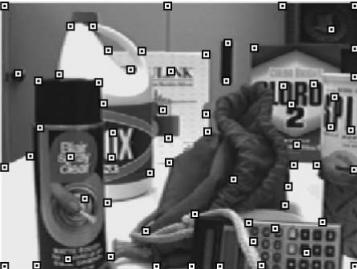
\includegraphics[width=0.32\linewidth]{Figures/points/harris.png}
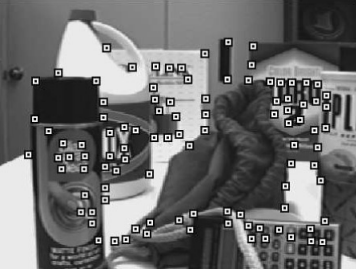
\includegraphics[width=0.32\linewidth]{Figures/points/klt.png}
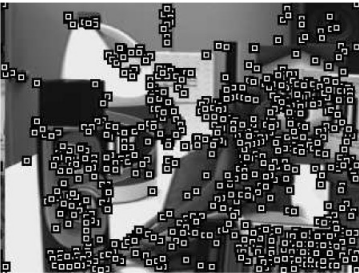
\includegraphics[width=0.32\linewidth]{Figures/points/sift.png}
}	
\end{figure}

\section{Challenges}

Object detection and tracking is still an open research problem in computer vision. A robust, accurate and high performance approach is still a great challenge. The level of difficulty depends on how the object of interest is defined in terms of features. For instance, Using color as object representation method, it is not difficult to identify all pixels with same color as the object. However, there is always a probability of existence a background region with same color information (background clutter). In addition, illumination changes in the scene does not guarantee that the pixel values of an object will be the same in all frames. These variabilities or challenges which are random in object tracking causes wrong object tracking, and are listed below.

\begin{itemize}
\item \textbf{Illumination Variation (IV):} It is desirable that background model adapts to gradual changes of the appearance of the environment.
\item \textbf{Scale Variation (SV):} Ratio between initial object size and current object size differs.
\item \textbf{Occlusion (OC):} Partially or full, occlusion affects the process of computing the background frame. In real life situations, occlusion can occur anytime the object of interest passes behind another object with respect to a camera.
\item \textbf{Dynamic background:} Some scenery regions contain movement, but should be still remain as background, acoording to their relevance. Such movement can be periodical or irregular, causing blurring (motion blur - MB), e.g. traffic lights, waving trees).
\item \textbf{Out of view (OV): } Some portion o the target leaves the view.
\item \textbf{Background clutter (BC):} As stated before, this challenge makes the segmentation task difficult. It is hard to create ans separate background model from moving foreground objects.
\item \textbf{Fast Motion (FM):} The speed of a moving object plays an important role in its detection and track. If an object is moving too slow, the temporal differencing methods fails to detect object, because it preserves uniform region between frames. In the other case, fast moving object leaves ghost regions in a detected foreground model.
\item \textbf{Object rotation and deformation (DEF):} Since natural objects move freely, they can appear slightly or completely transformed. Such rotations, in (IPR) or out (OPR) of plane on the images affect object tracking considerably.
\item \textbf{Low Resolution (LR):} Number of pixels inside the object bounding box is less than 400.
\end{itemize}

\section{Tracking Datasets}

In computer vision, a \textit{dataset} could be defined as a collection of images or video sequences used for testing algorithms. The amount of data and characteristics presented in the list, depend on the field that is studied. For instance, in scene recognition, a dataset contains images of landscapes or outdoor environments. Generally, this collection is shared between researchers and plays an important role in comparison and evaluation of state-of-the-art approaches.

The Surveillance Performance Evaluation Initiative (SPEVI) can be used for evaluating algorithms for surveillance-related applications. The first dataset contains 5 sequences applied to single person/face detection and tracking. The second dataset applies for multiple person/face detection and tracking. The sequences contain four targets occluding each other repeatedly. ETISEO dataset contains indoor and outdoor scenes, such as corridors, buildings entries, etc. This dataset can be used for surveillance applications.

PETS dataset became a surveillance project whose challenging scenarios are focused only on high level applications of this field. Some issues, like illumination or scale changes are not considered in these videos. Most of the sequences are used for person/vehicle tracking in outdoor environments(subway stations, building entrances). CAVIAR is a dataset used generally for situation recognition systems. However, sequences can be applied for tracking evaluation methods. Includes videos of people walking alone, meeting other people, entering and exiting shops.

The VIdeo Surveillance Online Repository (VISOR) database covers a wide range of scenarios and situations, including videos for human action recognition, outdoor videos for face detection, indoor videos for people tracking with occlusions, vehicles detection and surveillance. The VIdeo Surveillance Online Repository, includes several sequences for two separate tasks: First, an abandoned baggage scenario and second, a parked vehicle scenario.

In generic visual tracking, a dataset is a collection of videos that contains and object moving in some scenario. The sequences vary in length from hundreds of frames to thousands. Diverse object types are used. Different scene settings (indoor or outdoor, static or moving camera). Also different challenges, such as object occlusions or illumination conditions are presented. Most commonly used tracking benchmarks are summarized in table \ref{table:datasets}.  Recently, the authors in \cite{Wu2013b} released a benchmark containing 50 most commonly used sequences from some datasets mentioned \ref{table:datasets}, to facilitate fair performance evaluation. Also for better evaluation and analysis of strengths and weakness of tracking approaches. They classified sequences, considering a object tracking challenge, as a category, constructing several subsets to report specific challenging conditions. Some attributes occur more frequently, and some sequences are annotated with several attributes.

\begin{table}[h!]
\centering
\begin{tabular}{|ll|}
\hline
Name/Author/Paper & Sequences \\
Babenko           & 3         \\
Bobot             & 12        \\
Cehovin           & 5         \\
Ellis IJCV2011    & 3         \\
Godec             & 7         \\
Kalal             & 10        \\
Kwon              & 4         \\
Kwon VTD          & 11        \\
PROST             & 4         \\
Ross              & 4         \\
Thang             & 4         \\
Wang              & 4         \\
\hline
\end{tabular}
\caption{Popular object tracking datasets}
\label{table:datasets}
\end{table}

\section{Object Tracking}

The goal of an object tracker is to generate an object path over time. This trajectory consists of the object position over time in every frame of the video. The tracker may provide complete region in the image that is occupied by the object at every time instant. Certainly, this list is not meticulous and covers popular approaches on each category.

\subsection{Point Tracking}

Tracking can be formulated as the correspondence of objects represented by points across frames. This category can be divided into two subcategories:

\textbf{Deterministic Methods: } These approaches for point correspondence define a cost of associating each object in frame $t-1$ to a single object in frame $t$ using motion constraints, such as proximity, velocity, rigidity and motion. Minimization of the correspondence cost is formulated as a combinatorial optimization problem. A solution, which consists in one-to-one correspondence among all possible associations, can be obtained by optimal assignment methods. For instance Hungarian Algorithm \cite{Qin2012} or greedy search methods.

\textbf{Statistical methods for Point Tracking: } Statistical correspondence methods solve tracking problems whose measurements obtained from video sensors contain nose, or object motion can undergo random perturbations. These approaches take measurements and model uncertainties into account during object state estimation. Applying state space approach to model the object properties such as position, velocity and acceleration. In single object state estimation, tYhe optimal state of an object is giben by the Kalman Filter \cite{Ren2008a,Heikkila2004}, assuming measurement noise have a Gaussian distribution. In the general case, that is, object state is not assumed as Gaussian, estimation can be performed using particle filters \cite{Okuma2004,Rittscher2000}.

In the case of multiobject data association, state estimation using Kalman or particle filters, it is necessary to solve first correspondence problem before these filters can be applied. However, in cases when two objects are close each other, the correspondence could be incorrect. Then, an incorrectly associated measurement can cause the filter to fail to converge. In order to tackle this problem, Joint Probability Data Association Filtering (JPDAF) \cite{Schulz2003} and Multiple Hypothesis Tracking (MHT) \cite{Zulkifley2012} are two used techniques for data association.

\begin{figure}[t!!]
\centering
{
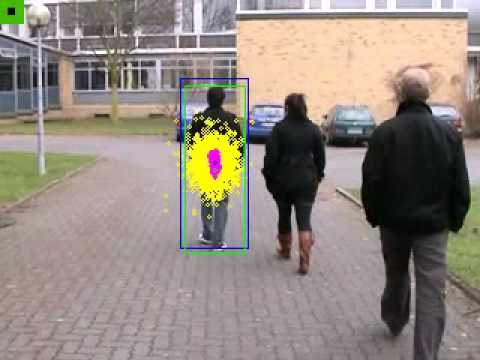
\includegraphics[width=0.32\linewidth]{Figures/particle_filter1.jpg}
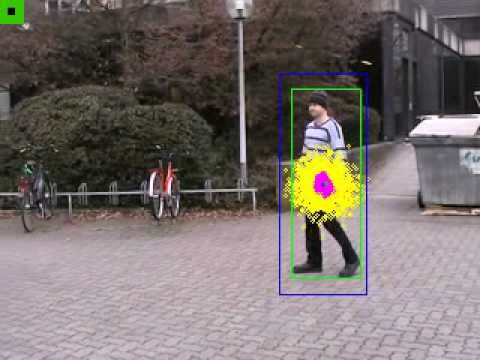
\includegraphics[width=0.32\linewidth]{Figures/particle_filter2.jpg}
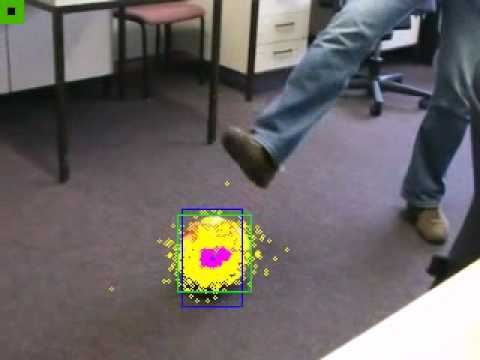
\includegraphics[width=0.32\linewidth]{Figures/particle_filter3.jpg}
}
\caption{\cite{Rittscher2000}}
\end{figure}


\subsection{Kernel Tracking}

In this type of tracking, object motion is computed using representations of a primitive object region, from one frame to the next. These algorithms differ in terms of appearance representation (features extraction) used, the number of objects tracked, and the method used for object motion estimation. 

\textbf{Density-based tracking:} According to \cite{Cheng1995}, the object is modelled with one or more probability density functions, such as Gaussian, mixture of Gaussian, Parzen windows or histogras, that describe the probability of object appearance. Mean-shift is an approach to feature space analysis. This method shifts a data point to the average of data points in its neighborhood. Mean shift uses fixed color distribution. A similar approach is called CAMSHIFT \cite{Exner2010} that handles dynamically changing color distribution by adapting the search window size and computing color distribution in the search window.

\textbf{Template-based tracking:}  These approaches apply templates of the object to calculate appearance probability on every frame of the video sequence. The most common is \textit{Template matching} \cite{Korman2013} that searchs accross the image, a region similar to the object template, defined in previous frames. The similarity measure is calculated using normalized cross correlation. A limitation of this method is its high computational cost due to brute force search. To reduce this cost, some methods limit the object search to a neighborhood near previous position.

Instead of templates, other object representations can be used for tracking. For example, color histograms or mixture models can be computed using the appearance of pixels inside the rectangular or ellipsoidal regions. To reduce computational complexitu, the similarity between object model and the hypothesized position, is computed evaluating the ratio betweem color means between model and position. The position with highest ratio is selected as current object location.

\begin{figure}[t]
	\centering
		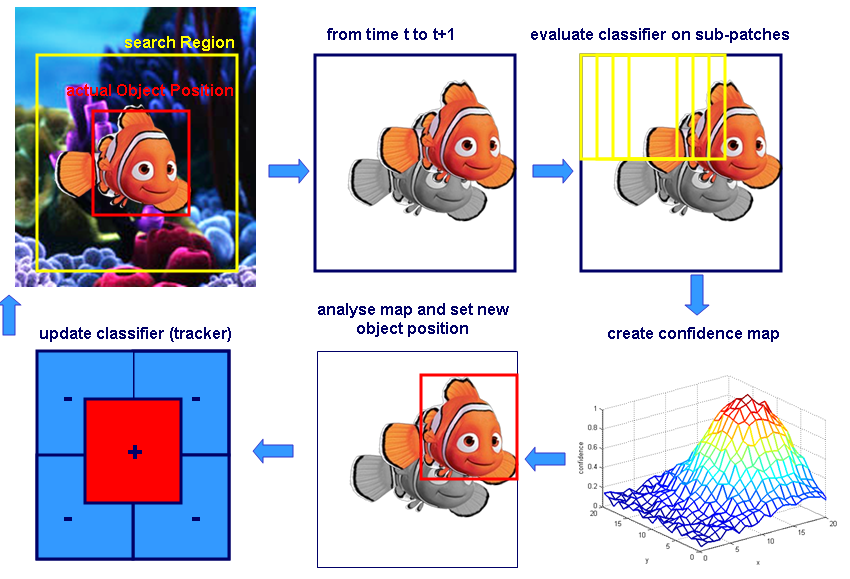
\includegraphics[width=0.7\linewidth]{Figures/overview_boost.png}
	\caption{Overview for online boosting object tracker}
	\label{fig::overview_boost}
\end{figure}	

"Tracking by detection" or "Tracking by repeated recognition" \cite{Mori2006} systems generally perform target object appearance learning. These methods are closely related to object detection (an area with great progress in computer vision) and has encouraged some successful real-time tracking algorithms \cite{Liu2007,Grabner2006}. However, many tracking algorithms employ static appearance models that are defined manually or trained at the first frame only \cite{Isard2001, Lepetit2006, Black1996, Comaniciu2000, Adam2006}, these methods are often unable to deal with significant appearance changes. This situations are difficult when there is limited knowledge of the object of interest. In order to cope this problem, an adaptive appearance model that changes during the tracking process as the appearance of the object changes, gets better results \cite{Ross2007,Matthews2004,Jepson2003}.

Boosting has been used in a wide field of machine learning tasks and applied to computer vision problems. Many tracking algorithms are based on the boosting framework \cite{Freund1997a} and is related to the work on Online Adaboost \cite{Avidan2007,Grabner2008,Oza2000}, multi-class boost \cite{Saffari2010} and MILBoost \cite{Babenko2010}. The goal of boosting is to combine many weak classifiers (usually decision stumps) into a linear strong classifier.


\subsection{Silhouette Tracking}

The object is tracked via estimation of the object region in each frame. Silhouette-based methods provide an accurate shape description for the objects that are tracked. These approaches can be divided into two main categories, shape matching and contour tracking. Shape matching \cite{Li2001} approaches search object silhouette in the current frame. Contour based, evolve initial contour to its new position in the current frame using state space models or direct minimization of some energy function \cite{Cremers2003}.

\begin{figure}[h!]
	\centering
		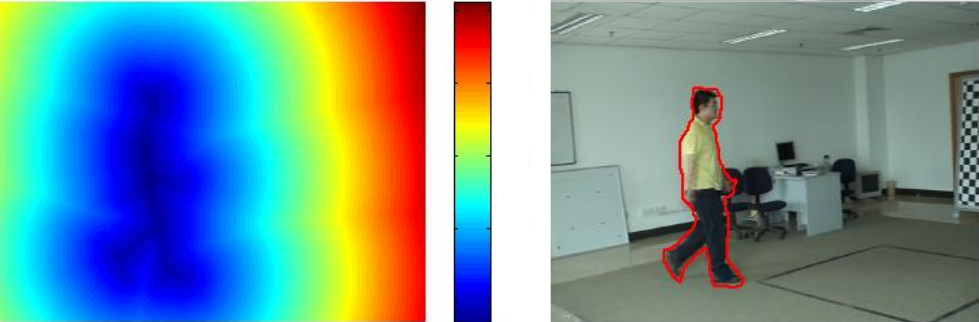
\includegraphics[width=0.9\linewidth]{Figures/contour.png}
	\caption{Illustration of an active contour representation. Left subfigure shows the signed distance map of a human contour; right image displays contour result.}
	\label{fig::contour}
\end{figure}	

\subsection{Tracking applying ensemble of trackers}

Several methods have proposed the use of ensemble classifiers within
the tracking-by-detection framework.
%The first algorithm that explicitly applies ensemble methods to
%tracking-by-detection is presented in \cite{Avidan2007}.
In this perspective, instead of ensembling the outputs of other trackers,
these methods focus on building ensemble classifiers,
such as Adaboost \cite{Avidan2007} or Bayesian probabilistic fusion \cite{Bai2013},
from weak low-level image features.
The classifier is then used to detect the target object in
new frames. Instead of working directly with low-level image features,
our ensemble tracker builds on top of tracker outputs
which are used as a more powerful mid-level representation of the target.
%Considering tracking as a binary classification problem, the author
%extends \cite{Collins2005} by using the Adaboost algorithm to
%combine a set of weak features and online updating of the object model.
%The classifier is then used to classify pixels in the next
%frames as either related to the object or background, which produces
%a confidence map of the location of the object.

Another alternative is to manually select a small set of trackers and use
prior knowledge on the behaviour of each tracker to build an ensemble.
In \cite{Santner2010a}, the authors combine a template-based tracker,
an optical flow tracker, and an online-random forest tracking-by-detection
method into a cascade.
In that case, the authors manually predefine a set of rules that decide
how to ensemble the tracker outputs. In contrast, our method can handle
a larger pool of trackers in the ensemble, since their outputs are combined
in a data-drive fashion that does not require manual rules or prior knowledge
on the behaviour of each tracker.
%The best selection is summarized into a simple
%set of rules. The authors explain that augmenting or updating in a smart way
%a simple online learner in terms of adaptivity can lead to much better results.


Sampling based approaches have also been explored for ensemble tracking.
Examples of this are the VTD \cite{Kwon2009} and
VTS \cite{Kwon2011a} trackers.
In this perspective, there is a sampling process that generates
multiple samples of target and tracker states. These trackers run in parallel
and their outputs are fused by probabilistic weighting. Therefore,
the ensemble uses a set of trackers of similiar architecture
with varying parameters. Our ensemble has the advantage of fusing outputs
of multiple trackers with no assumptions on their architectural similarity
and can leverage strenghts that different tracker architectures can provide.
%In these articles, the approaches obtain several samples of target and trackers
%states during sampling process using a Markov Chain Monte Carlo method.
%The trackers are sampled by proposing appearance models, motion models,
%state representation types, and observation types.
%Then, the sampled trackers run in parallel and interact with each other,
%covering target variations.

%The authors in \cite{Bai2013} proposed a classifier ensemble framework that
%uses Bayesian estimation theory to estimate the non-stationary distribution
%of sampled classifiers.
%In contrast with general tracking-by-detection classifiers,
%the weight vector that combines the classifiers is treated as a random
%variable and the posterior distribution of this vector is treated using
%Bayes' theory.
%Our approach presents a self-learning algorithm that enables
%object model updates based on tracking results and not from Bayesian updates of
%the classifier.

Finally, one can consider the case of offline fusion of trackers, such as in
\cite{Bailer2014}, where all trackers are applied to the entire sequence
and the ensemble is performed after the entire sequence is processed.
However, we are interested in the case of online tracking,
where the full sequence is not available beforehand. Furthermore, our online
approach is capable of steering and reinitializing failed trackers, increasing
the chances of better long-term tracking performance.

%the authors present an approach
%that merges the result of different tracking algorithms to produce a better
%tracking result.
%Based on the idea of attraction fields, which means the closer
%a fusion candidate is to a tracking result box,
%the stronger it is attracted by it.
%The result that maximizes the attraction of all trackers is chosen as a
%global result. In contrast, our fusion approach does not drop out bad tracking
%results. Our method is able to find and reinitialize outliers efficiently.
% Chapter Template

\chapter{Proposed Approach} % Main chapter title

\label{chapter4} % Change X to a consecutive number; for referencing this chapter elsewhere, use \ref{ChapterX}

\lhead{Chapter 4. \emph{Proposed Approach}} 

This section gives a detailed description of the implemented tracking system. Initially, giving an overview of the whole system and the basic functional blocks. Then, explaining implementation details of the different parts.

\section{The Tracking Loop}

Initially,  we explain the necessary building blocks of an object tracking system.

\section{Tracking system overview}

In order to tackle all the problems stated in the previous section, this tracking approach is separated into different modules.

\subsection{Basic overview}

Generic single-object tracking could be defined as the localization of an object through a video sequence. It is generic because the system is able to track any kind of object (faces, cars, etc.), and is single because the system will track just one object and not many at the same time. The proposed approach in this thesis is shown in \ref{fig::diagram}. Initially, our method starts with a pool of $n$ trackers $T = \left \{ t_1, t_2, ..., t_n \right \}$ and input data $\mathrm{x}$. This input corresponds to the initial rectangular box for an object in a sequence. All trackers are initalized and an updateable object model is created. Then, on each frame, our method runs and groups all trackers results by position into a set of $m$ clusters $C = \left \{ c_1, c_2, ..., c_m \right \}$. Also, we obtain a similarity measure which compares an actually tracking result patch to the current object model. The output should be the probabilities of similarity between the object model and each tracker result in that frame $S = \left \{ s_1, s_2, ..., s_n \right \}$. Using clustering information, the system can select between the winner cluster $c*$ which has the highest number of members, or the cluster with highest similarity measure. the others clusters are considered outliers and are reinitialized each 15 frames.

\begin{figure}[t!]
	\centering
		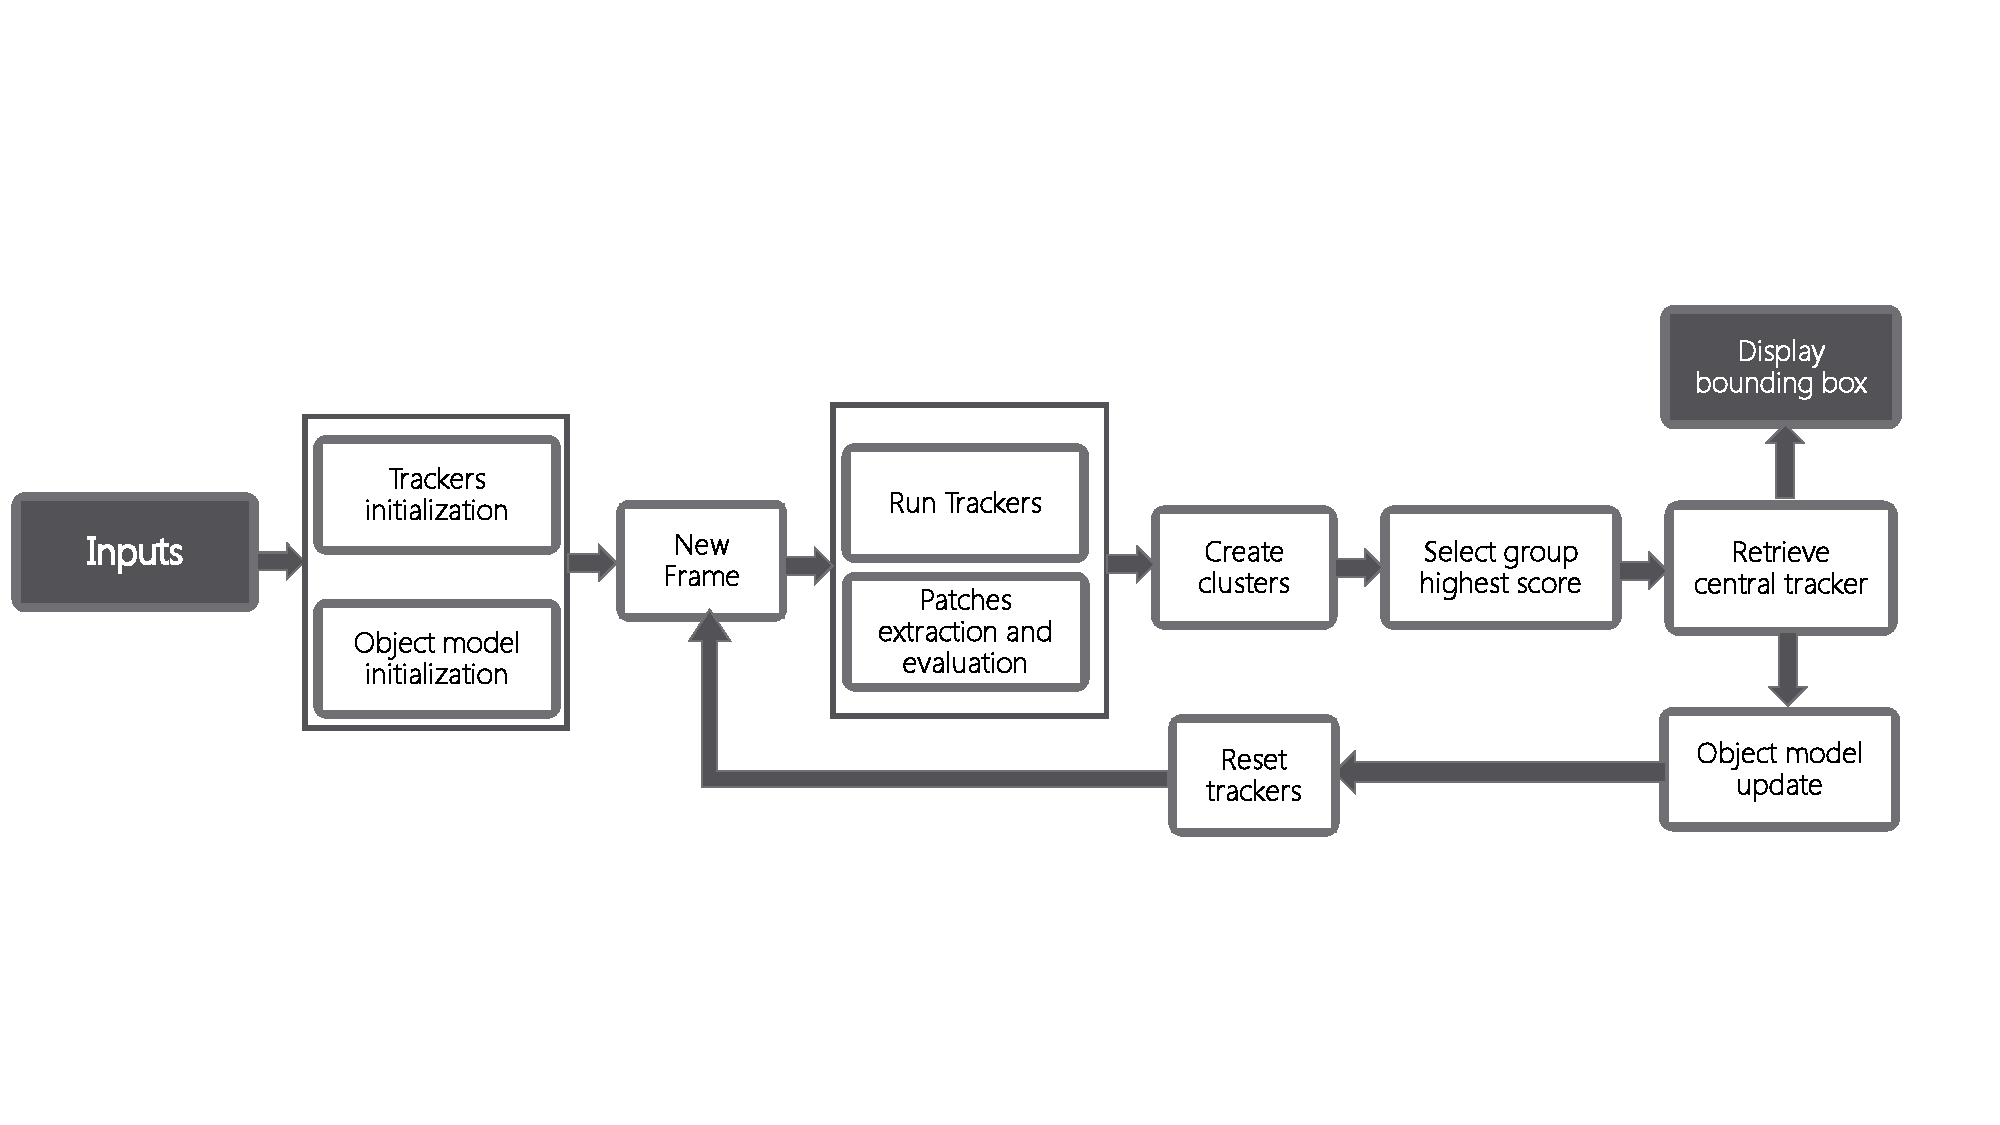
\includegraphics[width=1\linewidth, trim= 0cm 3cm 1cm 4cm, clip=true]{Figures/block_diagram.pdf}
	\caption{General schema for generic single-object tracking proposal.}
	\label{fig::diagram}
\end{figure}

\subsection{Trackers bounding boxes clustering}

Cluster analysis is the formal study of algorithms and methods for grouping, or classifying objects. These objects are described as a set of measurements or by relationships between the object and other objects. A \textit{cluster} is comprised of a number of similar objects collected or group together. Other authors define a cluster as a set of entities which are alike, and entities from different clusters are not alike, or "A cluster is an aggregation of points in the test space such that the \textit{distance} between any two points in the cluster is less than the distance between any point in the cluster and any point not in it". This theory is taken from \textbf{Jane and Dubes.}

Cluster analysis is the process of classifying objects into subsets that have meaning in the context of a particular problem. The objects are thereby organized into an efficient representation that characterizes the data. Clustering methods require that an index of proximity, or alikeness, or affinity, or association be established between pairs or patterns. A \textit{proximity matrix} $|d(i, j)|$ accumulates the pairwise indices of proximity in a matrix in which each row and column represents a pattern. Diagonal entries of a proximity matrix are ignored since all paterns are assumed to have the same degree of proximity with themselves. Also it is assmed that all proximity matrices are symmetric, so all pairs of objects have the same proximity index, independent of the order in which they are written.

A proximity index is either a \textit{similarity} or a \textit{dissimilarity}. The more the \textit{i}th and \textit{j}th objects are similar one another, the larger a similarity index and the dissimilarity index are.

Previous works show the common approach of data fusion using majority voting. The authors in \cite{Bailer2013} applied this method using a threshold parameter that defines if two result boxes vote for the same position. However, in \cite{Bailer2014}, the authors proved that this approach is sequence dependent. Instead, they settle the idea of attraction fields. We base our approach using the idea of clustering position. On a new frame, each tracker will give a rectangular box of where the object might be. Using this information, we are able to form groups of trackers that have similar positions. For each tracker result, we calculate the distance between its position and the rest of trackers running. The distance $d$ between two boxes $b$ and $c$ is computed as:

\begin{equation}
\large
d(b,c) = 1 - \frac{b\bigcap c}{b\bigcup  c}
\end{equation}

Using all distances, we construct a symmetric $l \times l$ proximity matrix $D$. We take the proximities to be dissimilarities. This means that $d(i,i) = 0$ for all $i$. We use complete-link hierarchical agglomerative clustering to form groups of trackers. Trackers $t_1$ and $t_2$ are "related" if their dissimilarity is below some threshold $v$. CL merges clusters in order of proximity; the closest clusters will be merged first, and the furthest clusters will be merged last. At each merge, CL creates a \textit{reduced proximity matrix}, with one less row and column. At the end, the algorithm delivers a set of clusters with size $m$ $C = \left \{ c_1, c_2, ..., c_m \right \}$ satisfying the following:
\begin{itemize}
\item $c_i \cap c_j = \emptyset$ for $i$ and $j$ from 1 to $m$, $i \neq j$
\item $c_1 \cup c_2 \cup ... \cup c_m = T$
\end{itemize}

\begin{figure}[t!]
	\centering
		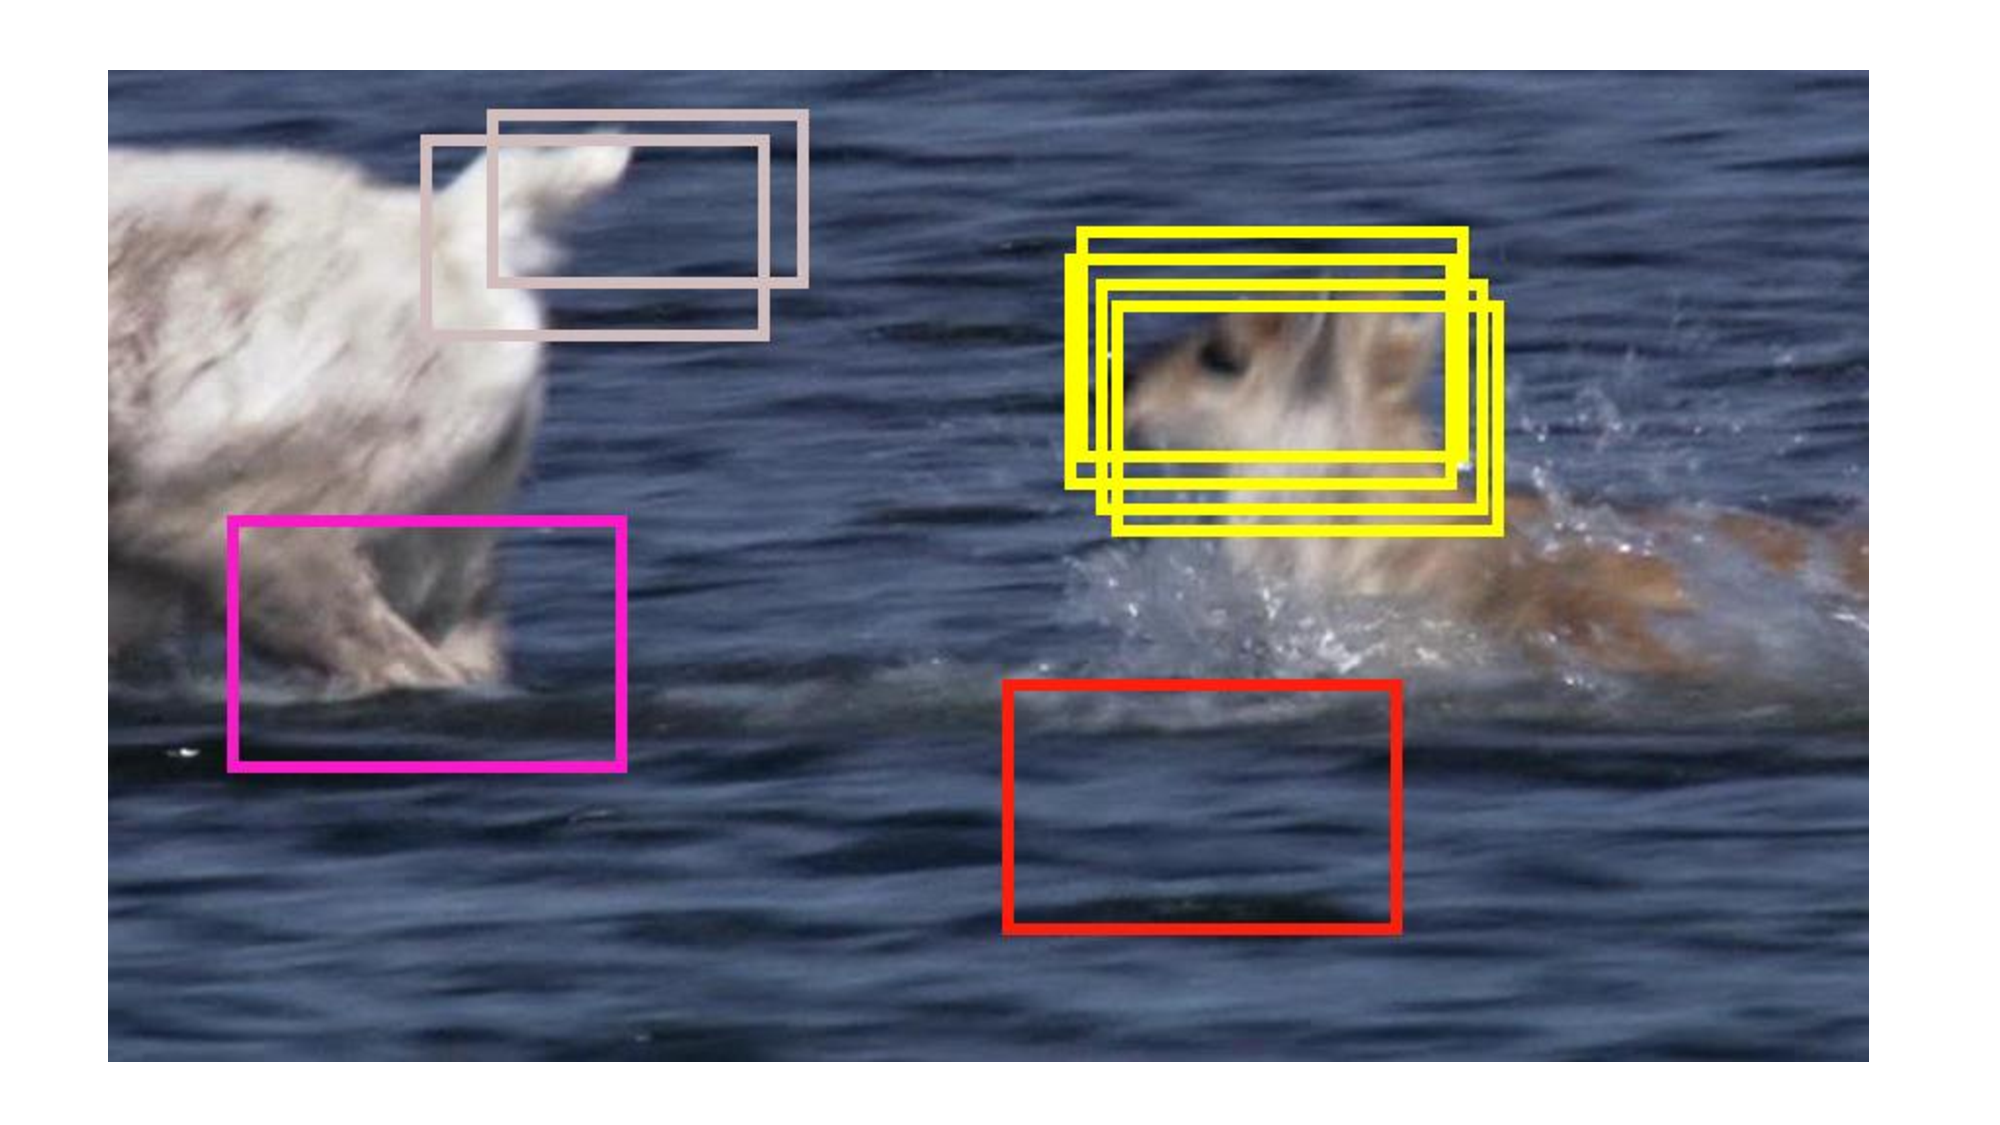
\includegraphics[width=0.65\linewidth, trim= 1cm 1cm 1cm 1cm, clip=true]{Figures/trackers_clustering.pdf}
	\caption{Tracking results clustering.}
	\label{fig::trackers_clustering}
\end{figure}

\subsection{Object modeling}

Visual object tracking has been formulated as a tracking-by-detection problem recently. In this case, object modeling is dynamically performed to support object detection in all frames. Mostly all approaches can be classified into two categories: \textit{Generative appearance models}, that mainly focus on how fit data into their correspondent object class; and \textit{discriminative appearance models}, that assume object tracking as a binary classification issue. The main goal is to maximize the separability between object and non-object regions discriminately.

Generally, Discriminative methods train a classifier using data acquired from previous frames, and subsequently use the trained classifier to evaluate possible object regions at the current frame (Figure \ref{fig::svm_example}). After localization, a set of \textit{positive} and \textit{negative} samples are heuristically selected to update the classifier. Some approaches apply online boosting \textbf{Cites}, that make a discriminative evaluation of features taken from a candidate feature pool, and then select the top ranked features to conduct the tracking process. Other methods apply Support Vector Nachines (SVM) method, which learns a margin-based discriminative appearance model, in order to maximize inter-class separability. It is important to note that these classifiers are trained using visual representations of the object.

\begin{figure}[t!]
		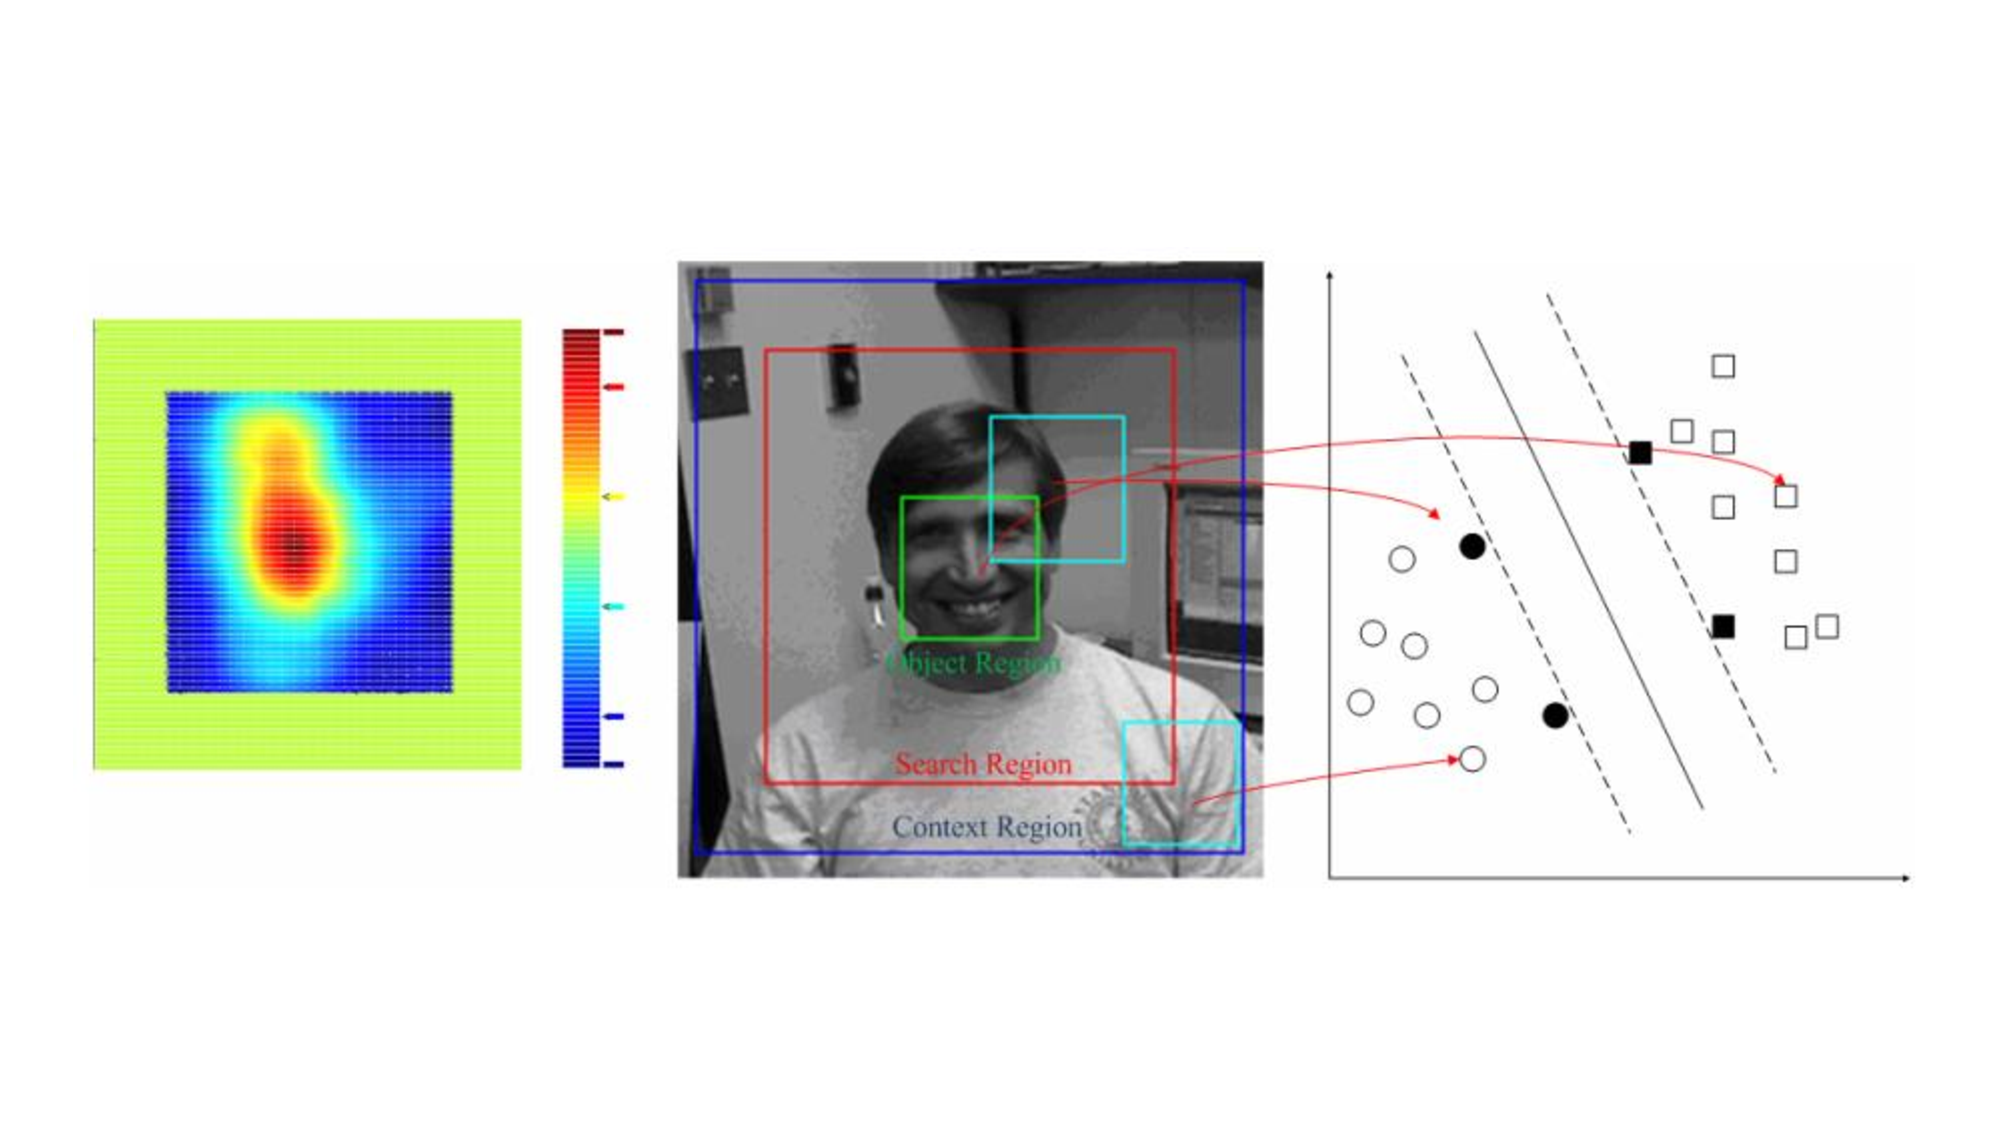
\includegraphics[width=1\linewidth, trim= 0cm 3cm 1cm 4cm, clip=true]{Figures/svm_example.pdf}
	\caption{Example of tracking-by-detection approach based on SVM classification. The left subfigure shows the score map of face and non-face classification; middle subfigure shows the search region for object localization and the context region for face and non-face samples selection; right subfigure plots the classification hyperplane that separates face and non-face classes.}
	\label{fig::svm_example}
\end{figure}


Tracking methods applying object appearence online learning have been recently applied. These systems discriminate object from its surrounding background through all the sequence using a classifier updated based on tracking results. However, these approaches except for MILBoost \cite{Babenko2010}, suffer from label jitter. The authors in \cite{Santner2010} explain that problem of label jitter arises if the bounding boxes of an object are not perfectly aligned with the target, although it is detected correctly. If label jitter occurs repeatedly over a tracking sequence, the tracker will most likely start to lose the target object. To cope this problem, we consider selecting a bag of trackers which share common similarity with appearance model.

The classifier corresponds to a standard linear SVM, which is trained with a buffer of 10 positives and 100 negative examples. The positive buffer is initialized using $\mathrm{x}$. We extract and image patch and calculate hog features. For the negative buffer we sample random bounding boxes with the same size on the image. During tracking, whenever a new example is added to the buffer, the classifier is retrained.


\subsection{Best cluster selection}

After perfoming clustering stage and obtaining classification scores with each tracker results, we can select the cluster that best follows the object. We present two selection criterias for best cluster.

\textbf{Best cluster selection based on members criteria:} Once groups are formed, we search the cluster $c^{*}$ in the list of clusters $C$ of size $m$, with highest number of trackers.

\begin{equation}
\large
c^{*} = \arg\max_{c\in C} ~\sum_{t \in c}t_{i} 
\end{equation}

\textbf{Best cluster selection based on appearance scores:} In this case we are considering classification scores for each cluster. Each cluster gives a score per cluster. Then, we select the winner cluster whose score is the highest one. 
\begin{equation}
\large
c^{*} = \arg\max_{c\in C} m_{i}
\end{equation}

where $m_i \in M = \left \{ m_1, m_2, ..., m_m \right \}$ corresponds to maximum score value of $c_i$ cluster:

\begin{equation}
\large
M =  \left \{ \max_{s\in S} s_i \in c_i \right \}
\end{equation}


\subsection{Best tracker selection}

The centered position $\mathrm{x}^{*}$ is selected by choosing the minimum sum of distances of the tracker, to the rest of trackers that belong to $c^{*}$. We did not consider selecting the tracker with best appearance score in order to avoid label jitter and drifting problems. Also selecting this value might make the tracker shaky.

\begin{equation}
\large
\mathrm{x}^{*} = \arg\min_{\mathrm{x}} ~\sum_{\mathrm{x}_{i} \in w^{*}}d(\mathrm{x_{i}}, \mathrm{x_{j}}) ,~~ i \neq j, \mathrm{x_{j}}\in c^{*}
\end{equation}

\begin{figure}[t!]
	\centering
		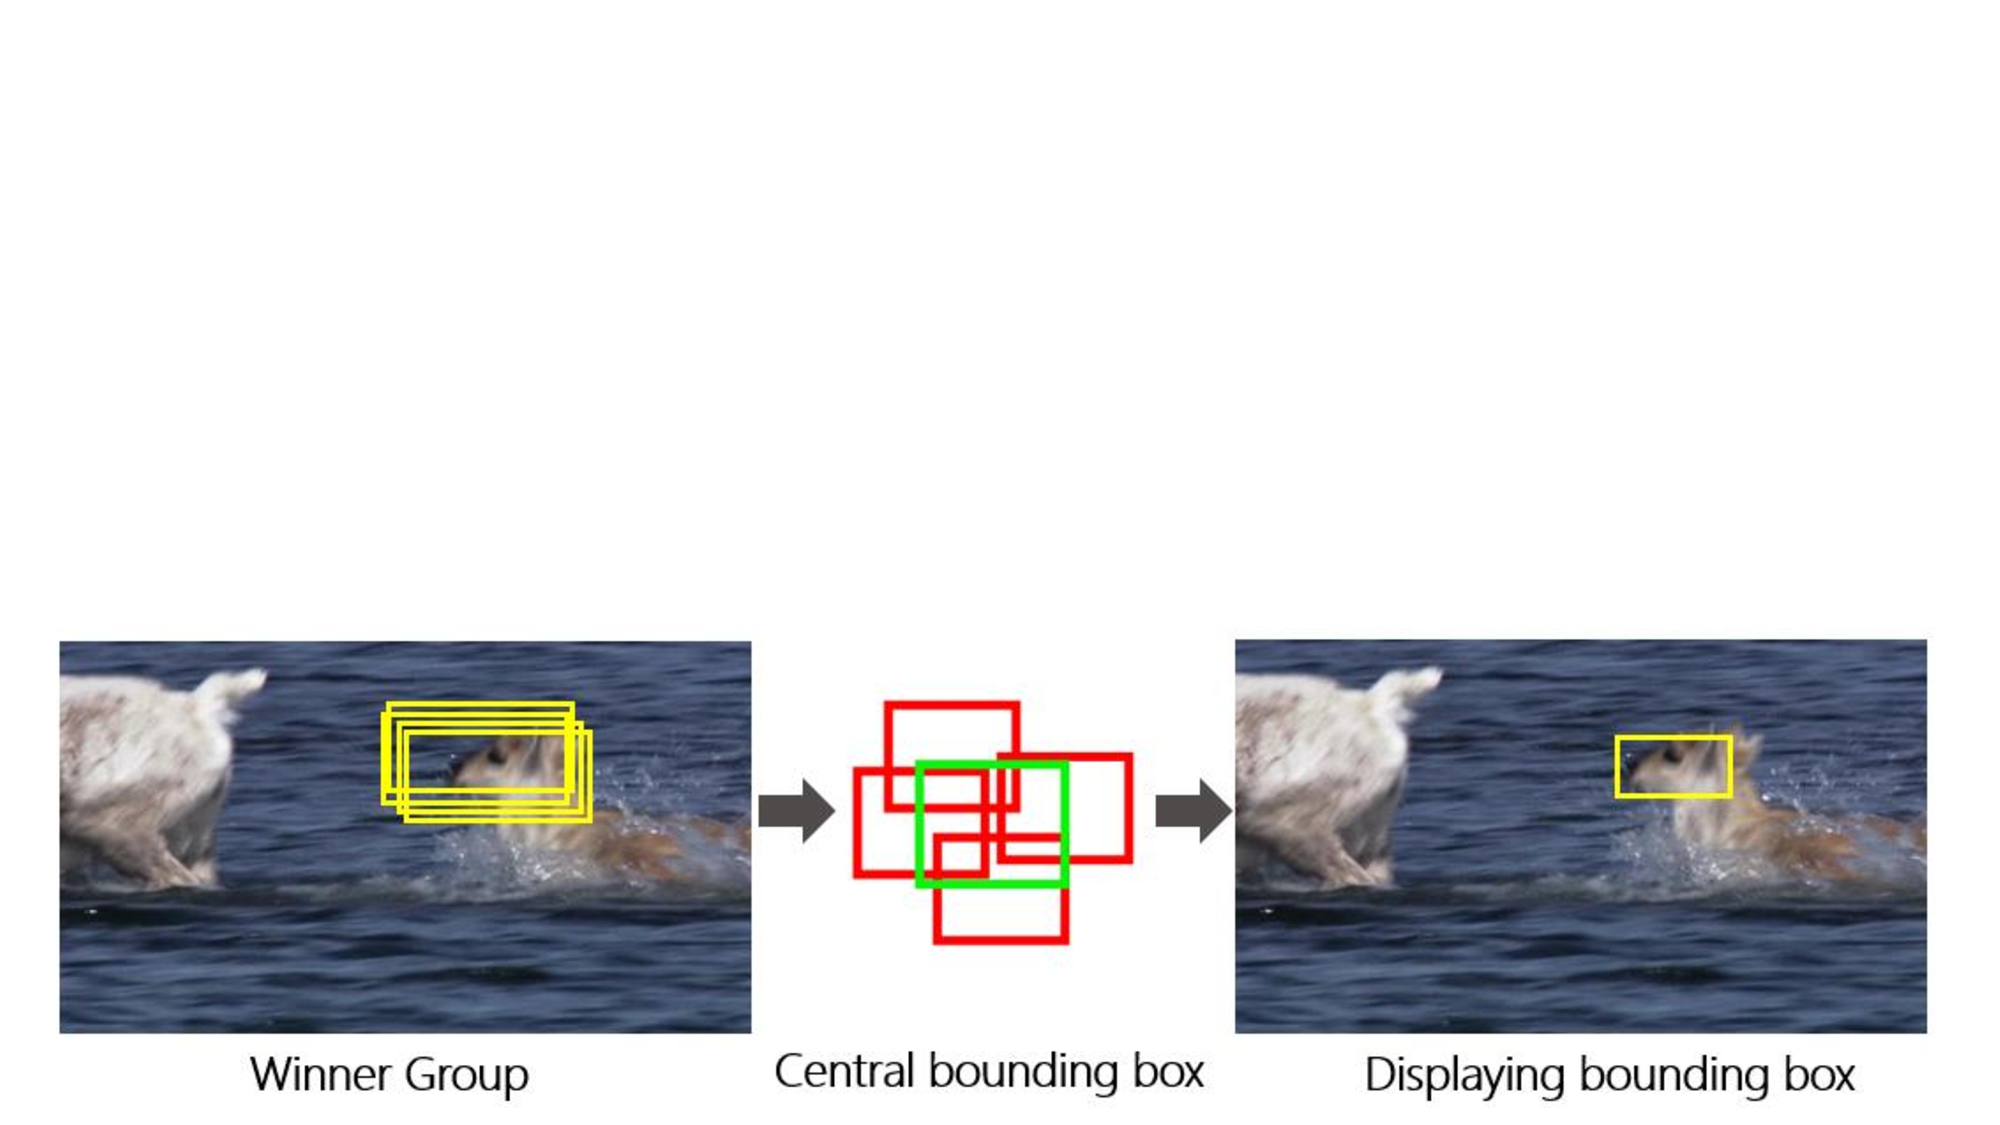
\includegraphics[width=0.95\linewidth, trim= 1cm 0cm 1cm 11cm, clip=true]{Figures/best_tracker.pdf}
	\caption{Best tracker bounding box selection.}
	\label{fig::best_tracker}
\end{figure}



\subsection{Trackers reset}

The outliers correspond to those trackers that does not belong to $c^*$. These trackers are reinitialized using $\mathrm{x}^{*}$. Also, from $\mathrm{x}^{*}$, we crop and image patch and extract hog features as new positive sample for the classifier.

\begin{equation}
\large
R = t_i \not\subset c^*
\end{equation}

\subsection{Object model update}

%\chapter{Experiments} % Main chapter title

\label{chapter4} % Change X to a consecutive number; for referencing this chapter elsewhere, use \ref{ChapterX}

\lhead{Chapter 4. \emph{Experiments}} 

In this section we report evaluations for our proposed approach. We compare our
tracking ensemble method and other state-of-the-art trackers using complete
50 sequences tracking benchmark \cite{Wu2013}. We also present qualitative and
quantitative analysis of our ensemble tracker, such as
individual performance of trackers and effect of the tracker pool.

\label{sec:experiments}

\begin{figure*}[t]
\centering
\subfloat{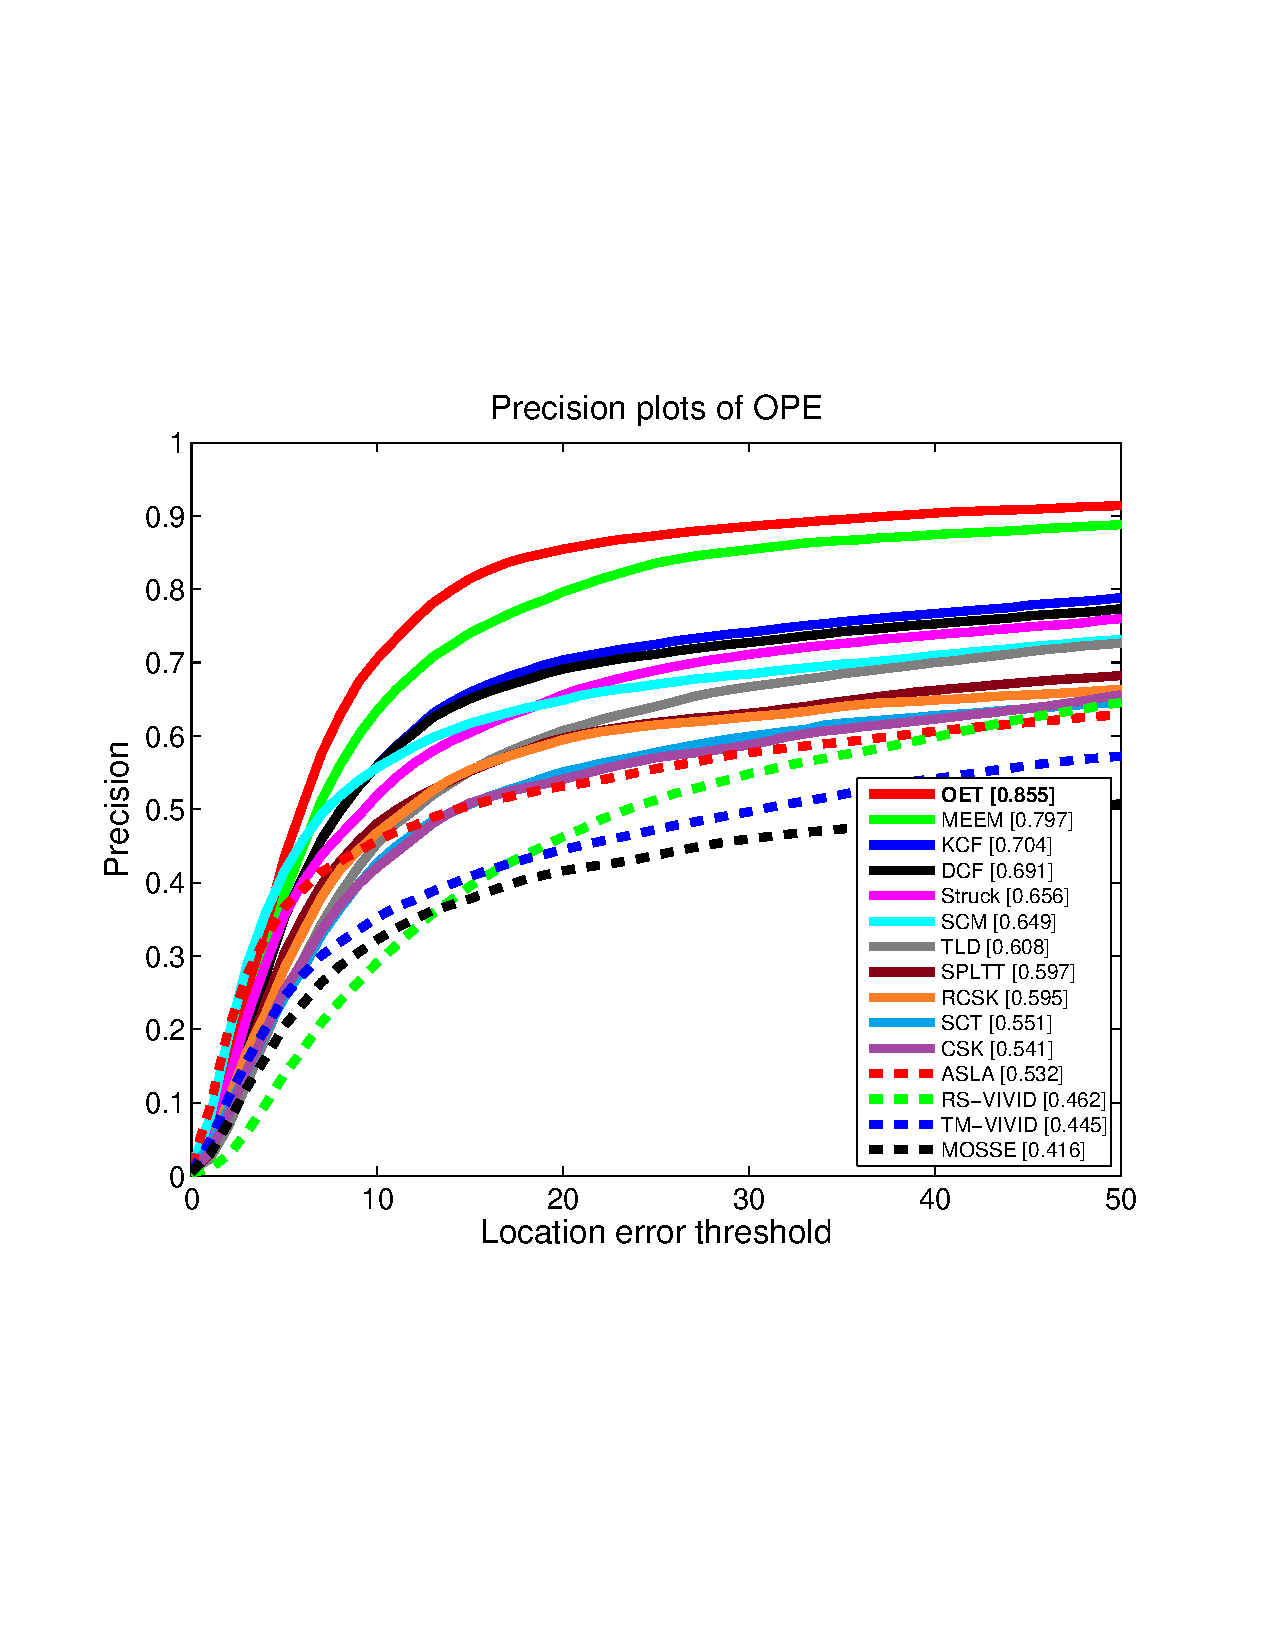
\includegraphics[width=0.5\linewidth, trim= 1cm 6.7cm 2cm 6cm, clip=true]{Figures/Results/quality_plot_error_OPE_threshold}
\label{fig:precision_plot}
}
\subfloat{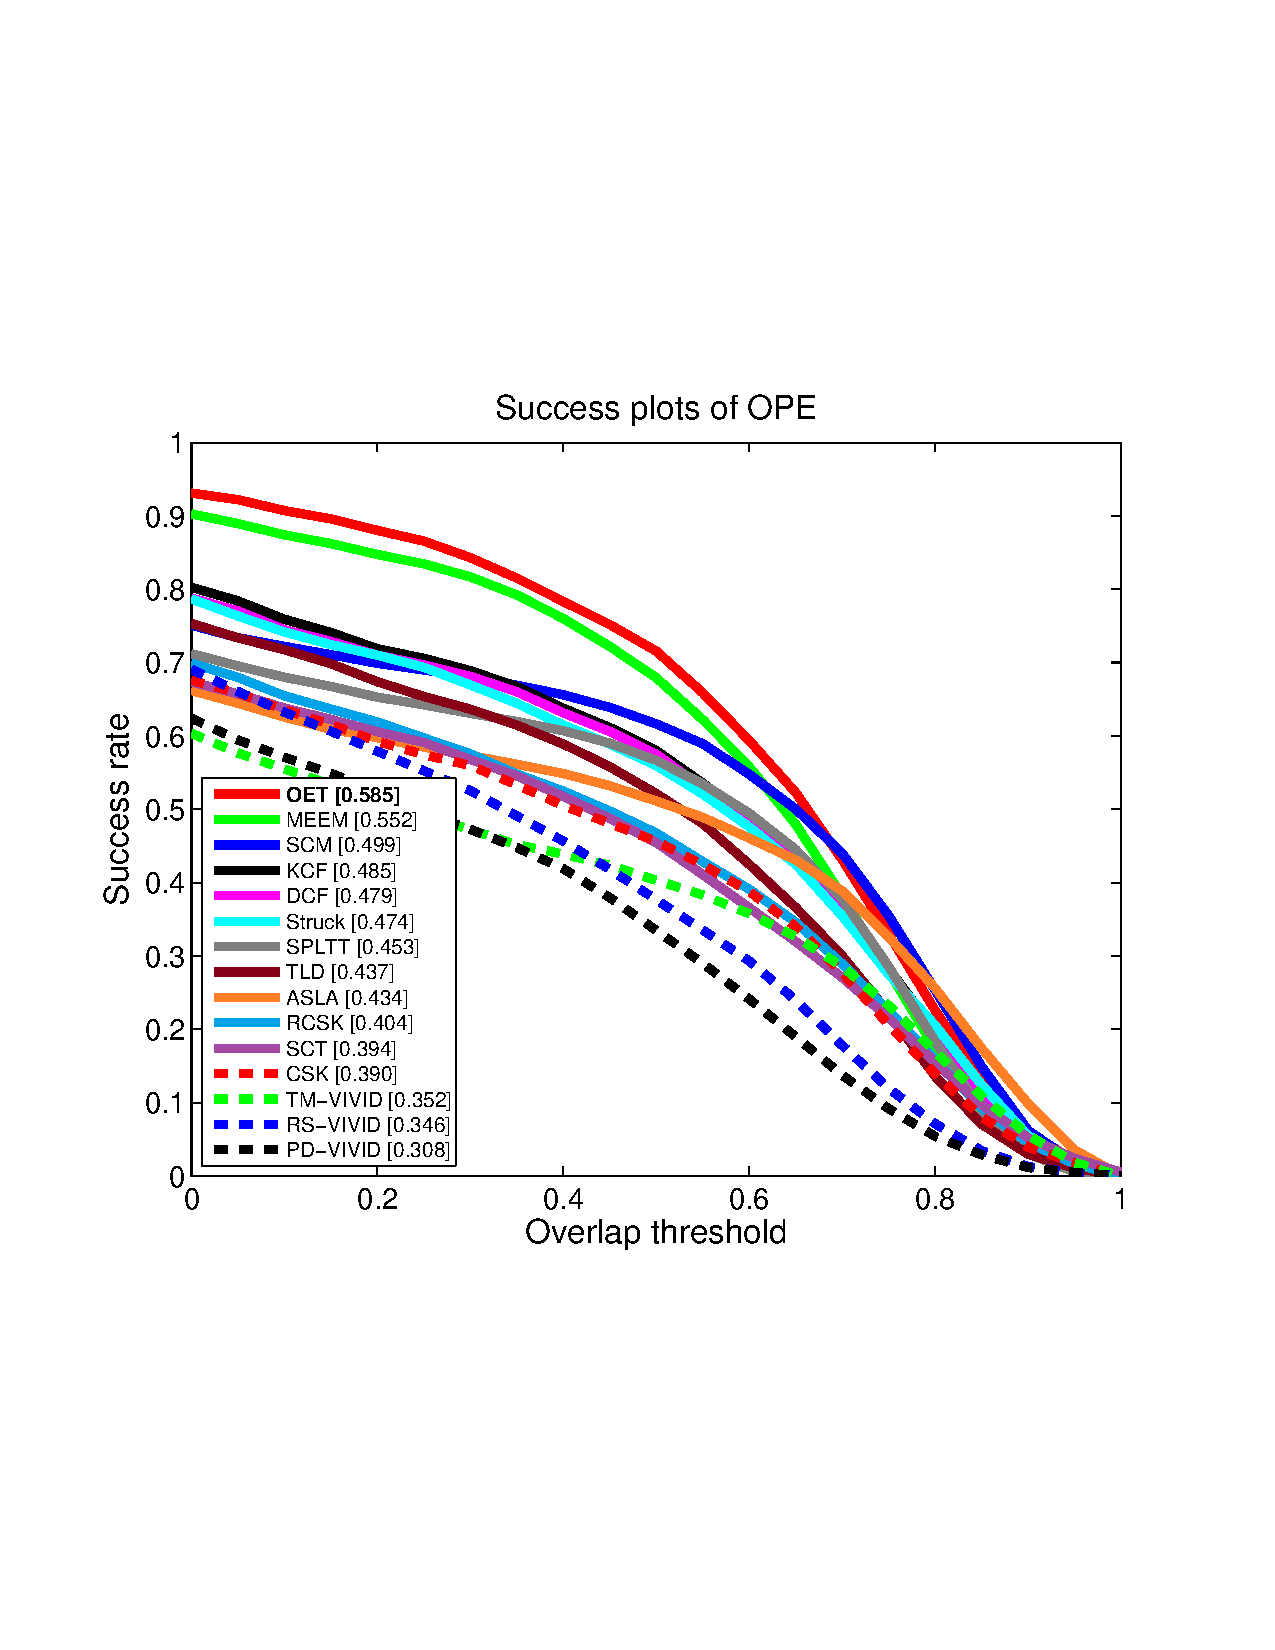
\includegraphics[width=0.5\linewidth, trim= 1cm 6.7cm 2cm 6cm, clip=true]{Figures/Results/quality_plot_overlap_OPE_AUC}
\label{fig:success_plot}
}
\caption{\small  Precision and success plots for all 50 sequences. Precision and success
		ratios are measured by center location error and overlap ratio,
		respectively. Trackers are ranked using scores of 20 pixels for
		precision and AUC for success.}
\label{fig:results}
\end{figure*}

\subsection{Experimental setup}
In order to evaluate the performance of our proposed ensemble tracking,
we adopt the Online Object Tracking Benchmark from \cite{Wu2013}.
This is an extensive benchmarking dataset that includes 50 sequences
annotated with 11 attributes.
The dataset includes challenging scenarios such as motion blur,
illumination changes, scale variation, occlusions,
in-plane and out-of-plane rotations, object deformation,
background clutter and low resolution.

We implement our online ensemble tracking algorithm in MATLAB.
All experiments are performed on desktop with an Intel Xeon CPU
and 16 GB of RAM.


\subsection{Evaluation Methodology}
To validate the performance of our proposed approach, we follow the one-pass
evaluation methodology (OPE) proposed in \cite{Wu2013}. 
We summarize the performance using the precision and success plots.

In
\textit{precision}, a frame is considered correctly tracked if the predicted
target center is within a distance threshold of the ground truth.
%In
%\cite{Henriques2014}, the authors explain that plotting the precision for all
%thresholds, no parameters are required. This makes the curves unambiguous and
%easy to interpret.
A higher precision at low thresholds means the tracker is
more accurate, while a lost target will not achieve perfect precision on a large
threshold range.
We rank tracking algorithms using their performance at 20 pixels
as in \cite{Babenko2010, Wu2013, Henriques2014}.

\textit{Success} measures intersection over union overlap between a tracker
output and a ground truth box and evaluates whether it exceeds a threshold.
%$t_H \in {0,1}$:
%\begin{equation}
%O(a,b) = \frac{|a\bigcap b|}{|a\bigcup  b|}
%\end{equation}
This overlap measure penalizes if the scale of the target is estimated incorrectly.
In contrast to precision, trackers are ranked using area under
the curve (AUC) metric, which relates to the average overlap across all frames. 

\subsection{Tracker pool}

\begin{figure*}[t!]
\centering
	\figuresr{subway/041}
	\figuresr{subway/042}
	\figuresr{subway/043}
	\figuresr{subway/044}
	\figuresr{subway/045} \\
	\figuresr{soccer/090}
	\figuresr{soccer/110}
	\figuresr{soccer/131}
	\figuresr{soccer/140}
	\figuresr{soccer/150}
\vspace{-2mm}
\caption{\small Qualitative results for object tracking applying both selection
	criterias in two sequences. \textbf{Green} bounding box corresponds to
	appearance score selection. \textbf{Blue} box to cluster size. In
	\textit{subway} when occlusion happens, many trackers are lost, creating a
	big cluster. In cases of background clutter \textit{soccer}, appearance
	selection loses target in some frames.}
\label{fig::clustvsapp}
\end{figure*}

We integrate into our pool tracking algorithms whose original source code
is publicly available.
%All trackers were modified in order to store their results and save
%their states on each frame.
Table \ref{table:trackers} shows the list of the
selected tracking algorithms. 

\begin{table}[h!]
\centering
\caption{\small Selected tracking algorithms for ensemble method. \textbf{Code Column}: 
M: Matlab, MC: Mixture of Matlab and C/C++, other: DLL files.}
\resizebox{\linewidth}{!}{%
\begin{tabular}{@{}p{9.5cm}ll@{}}
\toprule
 \textbf{Method}&  \textbf{Code}&  \\ \midrule
 Template matching - TM \cite{Collins2005a}&  other&  \\
 Mean Shift - MS \cite{Collins2005a}&  other&  \\
 Variance Ratio - VR \cite{Collins2005a}&  other&  \\
 Peak Difference - PD \cite{Collins2005a}&  other&  \\
 Ratio Shift - RS \cite{Collins2005a}&  other&  \\ 
 Adaptive Structural Local Sparse Appearance Model - ASLA \cite{Jia2012}&  MC& 
 \\  Compressive Tracker - CT \cite{Zhang2012a}&  MC&  \\
 Minimum Experts Entropy Minimization - MEEM \cite{zhang2014meem}&  MC&  \\ 
 Self-paced learning for long-term tracking - SPLTT \cite{Supancic2013}&  MC& \\ 
 Kernelized Correlation Filters - KCF \cite{Henriques2014}&  M&  \\ 
 Dual Correlation Filters - DCF \cite{Henriques2014}&  M&  \\  
 Spatio-temporal Context Tracker - SCT \cite{Zhang2013}&  M&  \\
 Circulant Structure Kernel - CSK, sKCF \cite{Henriques2014}&  M&  \\
 Robust CSK tracker - RCSK \cite{Danelljan2014}&  M&  \\  
 Minimum Output Sum of Squared Error - MOSSE \cite{Bolme2010}&  M&  \\ 
\bottomrule
\end{tabular}}
\label{table:trackers}
\end{table}


\subsection{Benchmarking results}

We report the performance of our ensemble tracking algorithm on the 50
benchmarking sequences in
Figure \ref{fig:results}.
The plots compare our approach with each individual tracker
in Table \ref{table:trackers} and state-of-the-art trackers: Struck tracker
\cite{Hare2011}, Sparse Collaborative Model (SCM) \cite{Zhong2012}, TLD tracker
\cite{Kalal2011}. Our online ensemble tracking algorithm is denoted \textit{OET}.

We note that our tracking ensemble improves performance over current
state-of-the-art tracking algorithms in the benchmark.
From Figure \ref{fig:results}, our method outperforms each individual tracking
score, in both precision and success.
When inspecting individial sequences, we note that 
out method handles better camera
rotation sequences, such as \textit{singer1, singer2, fish, car4}, unlike
the competing
MEEM tracker. Also, our ensemble method can overcome complete object occlusion. In
sequences where this situation happens \textit{jogging, david3}, KCF trackers
fails tracking the object. 

%Establishing a general comparison, performance of MEEM is comparable to ours.
%However,  MEEM tracker fails handling camera rotation as in  sequences. Also, KCF tracker bring good tracking results.
%But, KCF usually fails handling complete objects occlusion. It is good to note,
%as in \cite{Bailer2014}, in our system, scale is not determined. We are
%dependent of each separated tracker scale, and some trackers do not consider
%scale correction. Some of them apply initialization scale over all sequence.
%However, our method outperforms each individual tracker and state-of-the-art
%trackers in success plot, where scale is considered.

\subsection{Analysis of the tracking ensemble}
In this subsection, we focus on the relevance of the number of trackers in the pool.
We vary the size of the tracker pool in order to evaluate its effect on the
performance of the ensemble.
When selecting small tracker pools, we first chose the best 5 trackers
from Fig.~\ref{fig:success_plot}. We then augment the pool with the next 5 trackers to
form a pool of size 10. Finally we add the worst 5 trackers for a pool of size 15.
%Finally, we add 5 last trackers.
We also study the effect of the inlier selection criteria of Section
\ref{sec:inliers}
(appearance score and cluster size).


\begin{table}[h!]
\caption{\small Average AUC and precision for live fusion methods tested in 50 videos
		dataset.}
\resizebox{\linewidth}{!}{%
\begin{tabular}{llll}
\hline
\textbf{Method}     & \textbf{\# trackers} & \textbf{Success(AUC)} & \textbf{Precision(20px)} \\
\hline
           & 5                  & 0.585        & 0.855           \\
\textbf{Appearance score} & 10                 & 0.569        & 0.811           \\
           & 15                 & 0.560         & 0.804           \\
\hline           
           & 5                  & 0.528        & 0.765           \\
\textbf{Cluster size}    & 10                 & 0.493        & 0.715           \\
           & 15                 & 0.480         & 0.678           \\
\hline
\end{tabular}}
\label{table:trackers_number}
\end{table}

The results are summarized in Table \ref{table:trackers_number} for all 50
sequences in the benchmark.
We report AUC ranking score for success, 
and 20-pixel threshold for precision.
%
%Table \ref{table:trackers_number} summarizes quantitative evaluation results for
%all 50 sequences.
%
Our algorithm generally outperforms other methods using
appearance score selection criteria. In case of cluster size selection,
this method usually fails handling occlusions. In some sequences, many trackers
lose object target and keep steady when occlusion happens, creating a big
cluster which has the biggest number of members (Figure \ref{fig::clustvsapp}).
However, this method is smoother and handles better fast motion and background
clutter sequences.

\begin{figure}[h!]
\centering
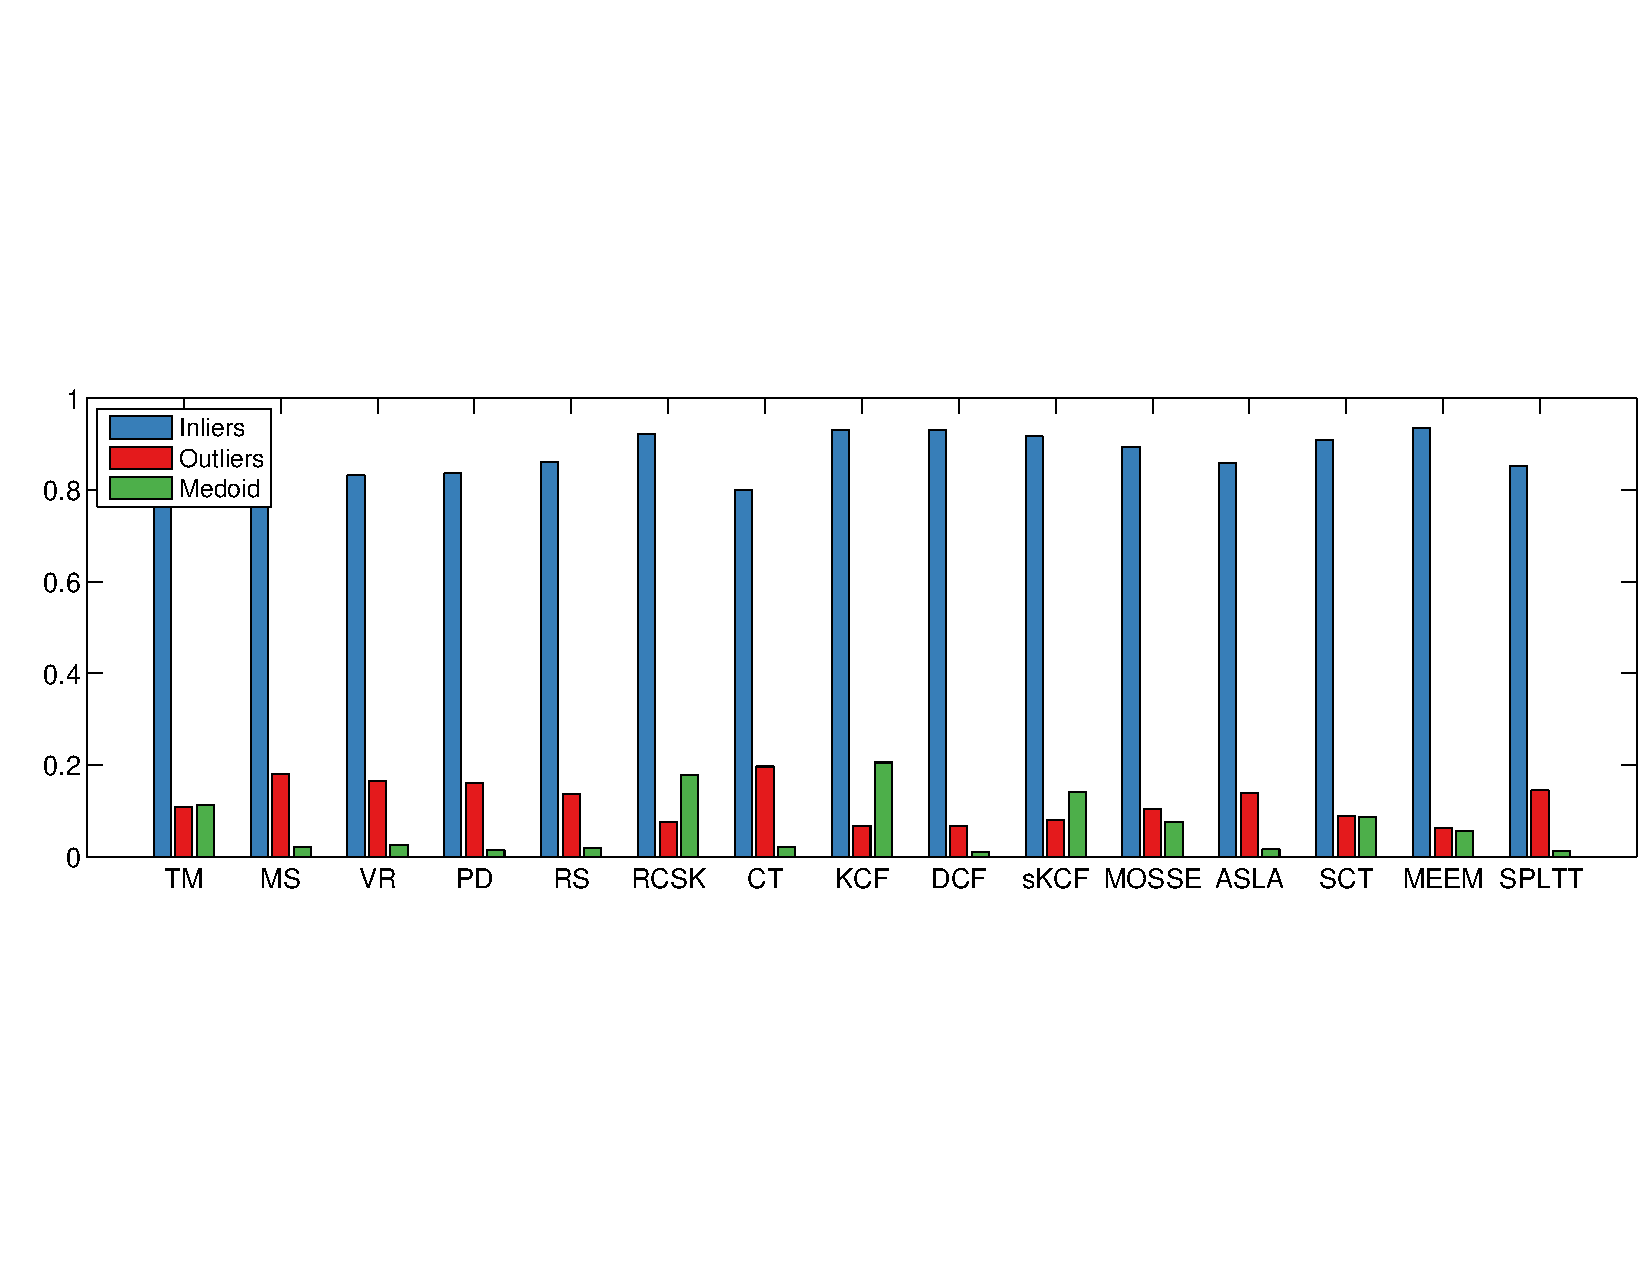
\includegraphics[width=1.0\linewidth, trim= 0.7cm 7.6cm 0.3cm 7.8cm, clip=true]{Figures/stats.pdf}
\caption{\small Statistics for each tracker in the ensemble over all frames. }
\label{fig:stats}
\end{figure}

\begin{figure*}
\centering
\subfloat[bolt sequence.]{
	\figuresall{bolt/015}
	\figuresall{bolt/196}
	\figuresall{bolt/236}
	\figuresall{bolt/316}
	\figuresall{bolt/346}	
}

\vspace{-0.3cm}

\subfloat[jogging-2 sequence.]{
	\figuresall{jogging-2/033}
	\figuresall{jogging-2/071}
	\figuresall{jogging-2/104}
	\figuresall{jogging-2/258}
	\figuresall{jogging-2/305}	
}

\vspace{-0.6cm}

\subfloat[singer-1 sequence.]{
	\figuresall{singer-1/048}
	\figuresall{singer-1/131}
	\figuresall{singer-1/179}
	\figuresall{singer-1/242}
	\figuresall{singer-1/306}	
}

\vspace{-0.45cm}

\subfloat[football sequence.]{
	\figuresall{football/005}
	\figuresall{football/086}
	\figuresall{football/135}
	\figuresall{football/325}
	\figuresall{football/353}	
}

\vspace{-0.55cm}

\subfloat[singer-2 sequence.]{
	\figuresall{singer-2/029}
	\figuresall{singer-2/069}
	\figuresall{singer-2/155}
	\figuresall{singer-2/211}
	\figuresall{singer-2/309}	
}

\vspace{-0.65cm}

\subfloat[skating1 sequence.]{
	\figuresall{skating1/058}
	\figuresall{skating1/093}
	\figuresall{skating1/237}
	\figuresall{skating1/295}
	\figuresall{skating1/329}	
}

\vspace{-0.25cm}

\subfloat[david3 sequence.]{
	\figuresall{david3/072}
	\figuresall{david3/092}
	\figuresall{david3/197}
	\figuresall{david3/218}
	\figuresall{david3/242}	
}\\
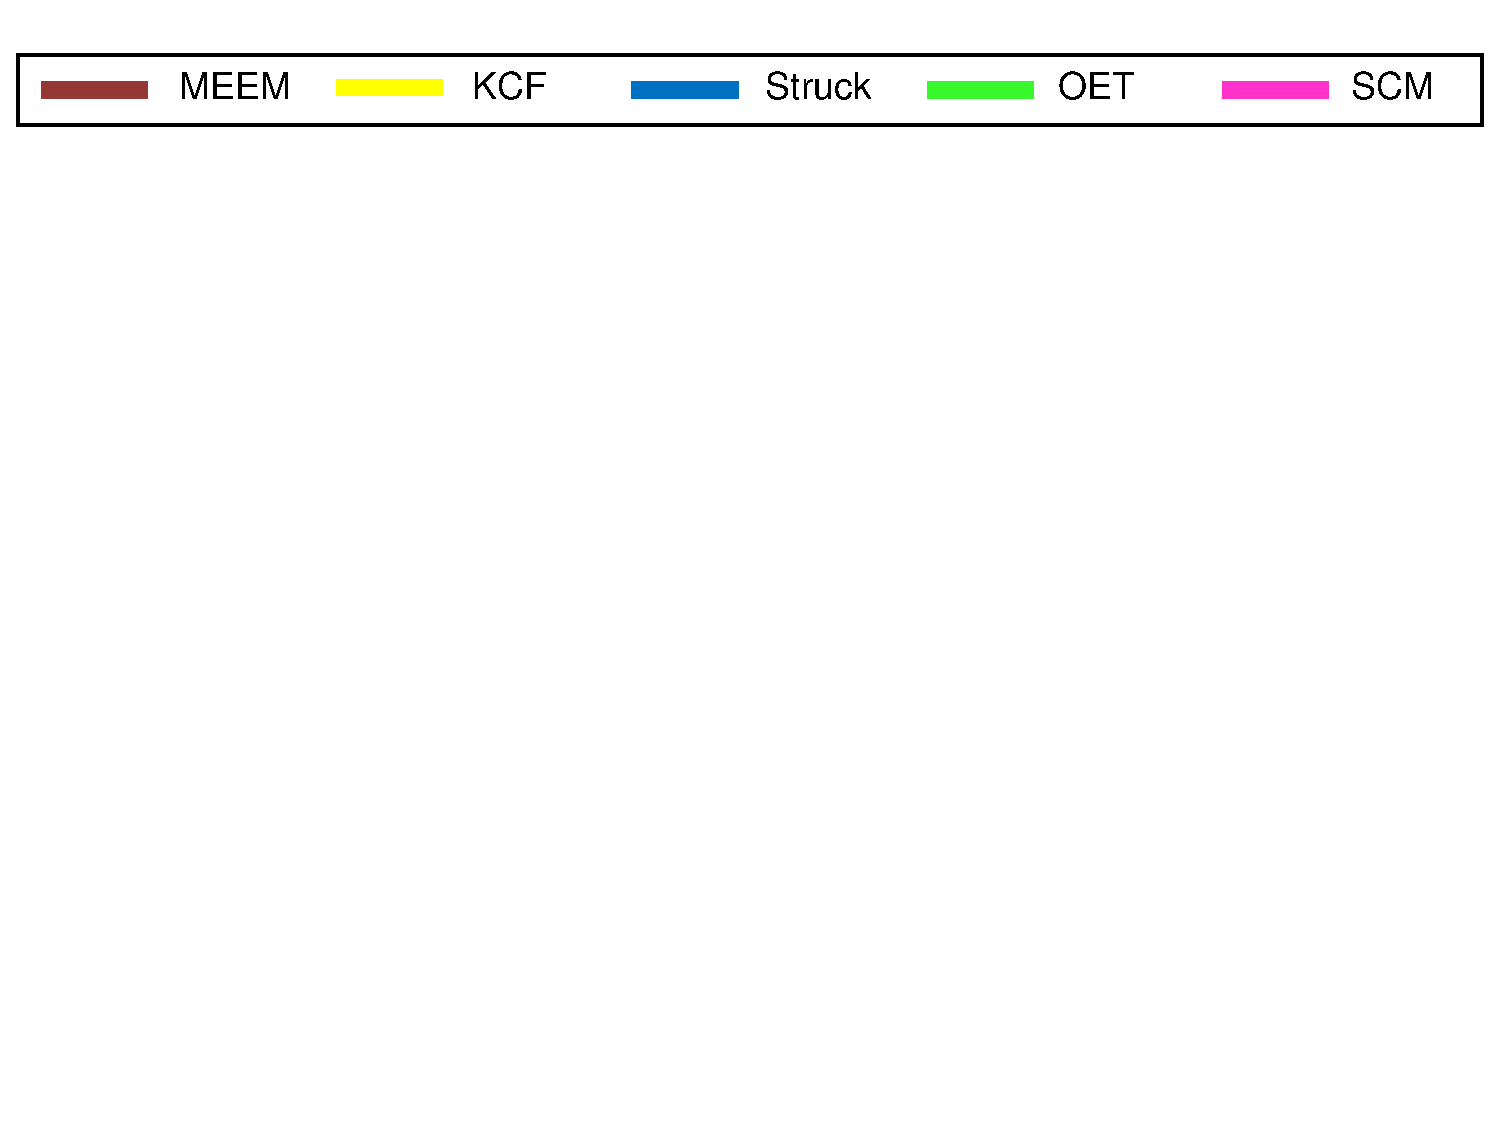
\includegraphics[width=0.8\linewidth, trim= 0cm 16cm 0cm 0cm, clip=true]{Figures/results_all/legend}
\vspace{-0.25cm}
\caption{\small Screenshots of tracking results.}
\end{figure*}

\begin{figure*}
\centering
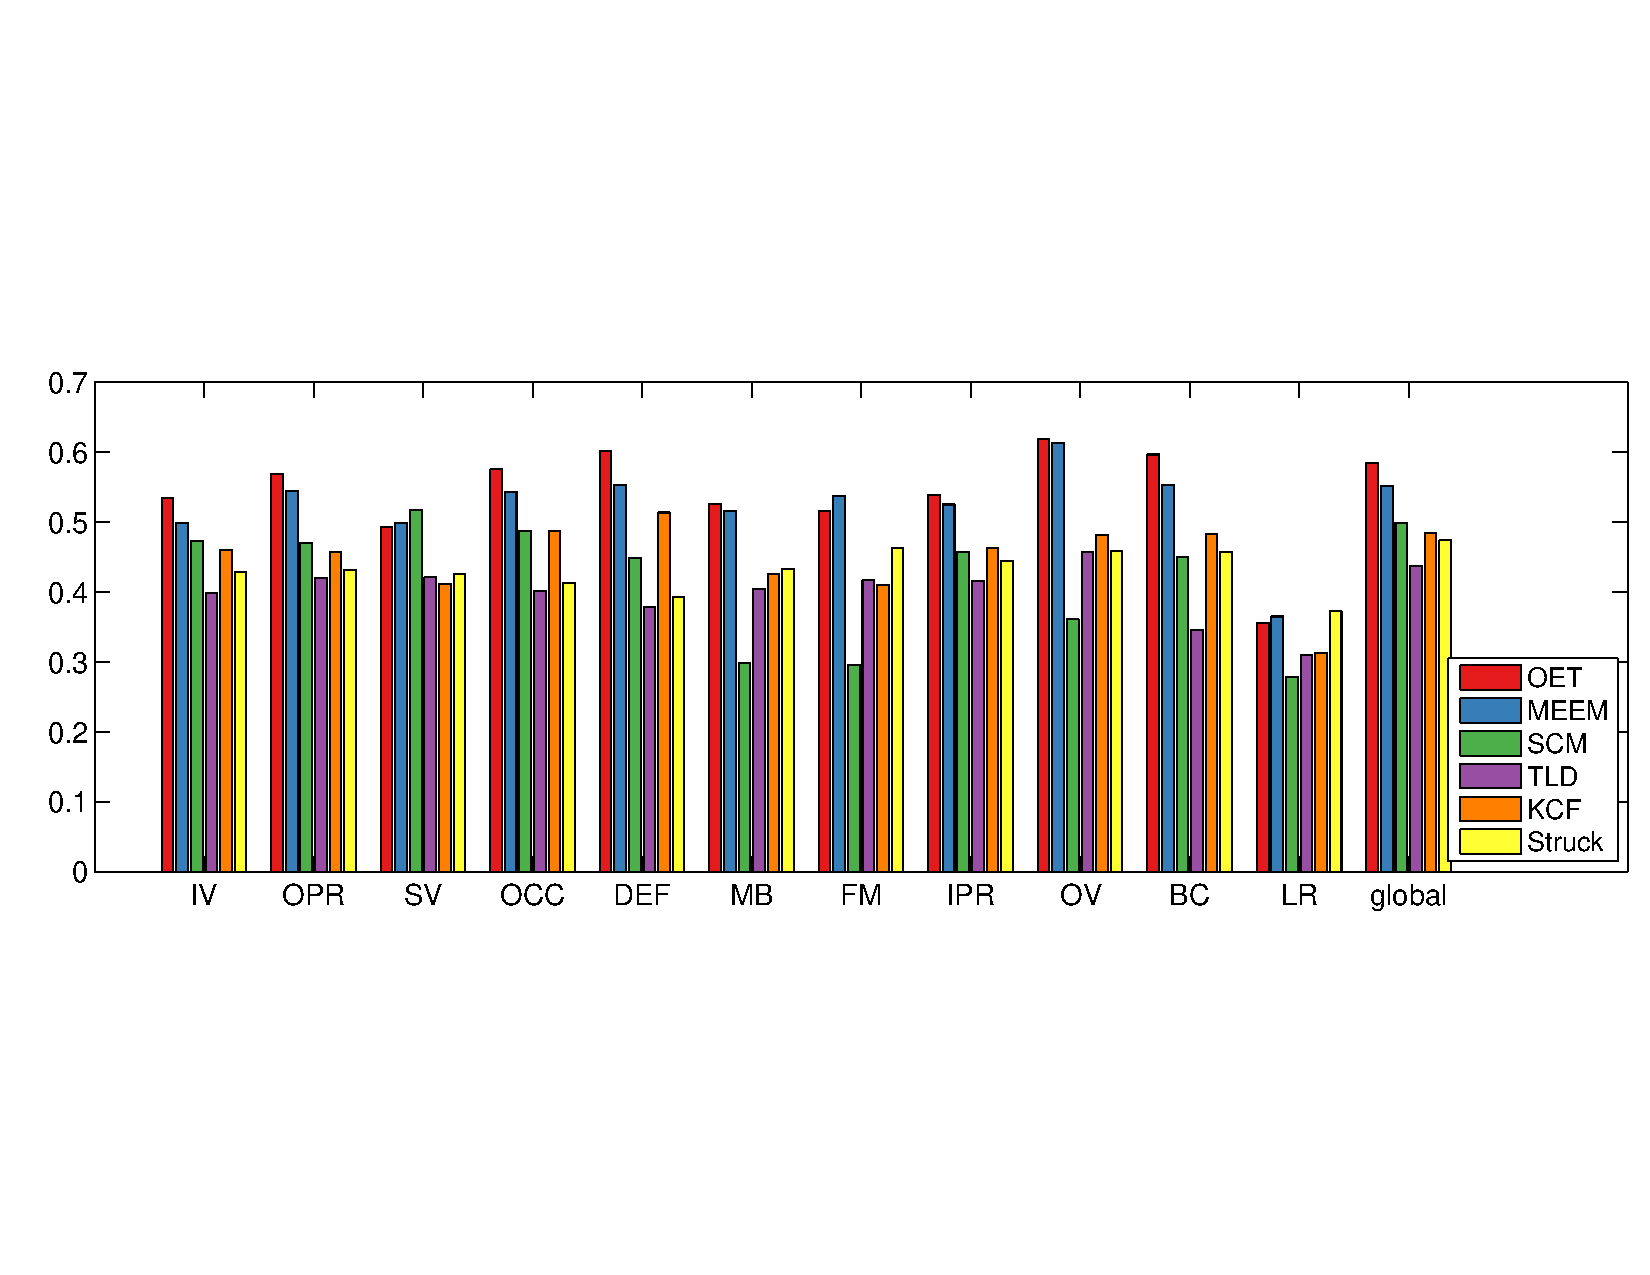
\includegraphics[width=1.0\linewidth, trim= 0.2cm 6.15cm 0.2cm 5.8cm, clip=true]{Figures/bar_graph.pdf}
\caption{\small Average AUC ranking scores of top trackers on different subsets of test
		sequences in OPE. Each subset of sequences corresponds to an attribute:
		IV - illumination variation, OPR - out of plane rotation, SV- scale
		variation, OCC - occlusion, DEF - deformation, MB - motion blur, FM -
		fast motion, IPR - in plane rotation, OV - out of view, BC - background
		clutter, and LR - low resolution. Average AUC for all 50 videos is
		presented as global.}
\label{fig:attributes}
\end{figure*}


We also note that adding trackers with lower performance hurts the ensemble.
However, the drop in performance when adding
weaker trackers, is less than 5\% ($\sim$300 frames) in success and 10\% in
precision ($\sim$500 frames). For instance, when performing inlier selection using
the
appearance score criteria, a spurious tracker may focus on a region with
very similar apperance to the object, \eg background clutter, which can
make tracking fail.
This is very common in the \textit{soccer} and \textit{shaking}
sequences.

In terms of running time, the average time cost for our ensemble
method is $0.062$ s/frame for 5
trackers, $0.122$ s/frame for 10 trackers, and $0.198$ s/frame for 15 trackers.
These timings do not include the processing time of each tracker.
%didn't consider each tracker processing time and model update for timing.

On the other hand, we present statistics about how often trackers in the pool
are selected as outlier, inliner, and medoid.
In figure
\ref{fig:stats}, for each tracker, there are 3 bars: percentage of frames that a
tracker was in best cluster(inlier - blue bar); percentage of frames where a
tracker was considered outlier (red bar); finally, percentage of frames that a
tracker was selected as medoid bounding box (green bar). Based on this result,
trackers whose individual performance is very high, have low percentage of being
considered outliers (KCF, MEEM, RCSK). MEEM individual performance is very high.
However, it does not have the highest frame percentage of being selected as
central bounding box, in comparison with KCF or RCSK. Also, trackers that were
considered spurious in previous experiments, have high rate in outliers bar
(MS, VR, PD, RS). 

\subsection{Experiments with sequence attributes}

The videos in the benchmark dataset are organized and selected with attributes,
which describe challenges present in the sequence - \eg occlusion, object
deformations. These properties are useful for diagnosing tracking behavior,
without the need of analyzing each video separately. Figure \ref{fig:attributes}
shows AUC ranking scores of recent trackers on different sequences, grouped by
attributes. For instance, background clutter (BC) contains all sequences whose
target pixels might be confused with background.

From figure \ref{fig:attributes}, our approach using appearance selection
outperforms other trackers in 8 of 11 attributes. Specifically, in attributes
such as IV (illumination variation), OPR (out of plane rotation), OCC
(occlusion), DEF (deformation), MB (motion blur), IPR (in plane rotation),
OV (out of view), and BC (background clutter). It is important to note that SCM
tracker is better than most recent trackers in terms of scale variation.
Results show that its affine motion models handle scale
variation better than other trackers, which are designed to account
translational motion \cite{Wu2013}. In our system, scale is not determined. We are
dependent of each separated tracker scale, and some trackers do not consider
scale correction. Some of them apply initialization scale over all sequence.

%\input{Chapters/Chapter2} 
%\input{Chapters/Chapter3}
%\input{Chapters/Chapter4} 
%\input{Chapters/Chapter5} 
%\input{Chapters/Chapter6} 
%\input{Chapters/Chapter7} 

%----------------------------------------------------------------------------------------
%	THESIS CONTENT - APPENDICES
%----------------------------------------------------------------------------------------

\addtocontents{toc}{\vspace{2em}} % Add a gap in the Contents, for aesthetics

\appendix % Cue to tell LaTeX that the following 'chapters' are Appendices

% Include the appendices of the thesis as separate files from the Appendices folder
% Uncomment the lines as you write the Appendices

%% Appendix A

\chapter{Appendix Title Here} % Main appendix title

\label{AppendixA} % For referencing this appendix elsewhere, use \ref{AppendixA}

\lhead{Appendix A. \emph{Appendix Title Here}} % This is for the header on each page - perhaps a shortened title

Write your Appendix content here.
%\input{Appendices/AppendixB}
%\input{Appendices/AppendixC}

\addtocontents{toc}{\vspace{2em}} % Add a gap in the Contents, for aesthetics

\backmatter

%----------------------------------------------------------------------------------------
%	BIBLIOGRAPHY
%----------------------------------------------------------------------------------------

\label{Bibliography}

\lhead{\emph{Bibliography}} % Change the page header to say "Bibliography"

\bibliographystyle{unsrtnatNEW} % Use the "unsrtnat" BibTeX style for formatting the Bibliography

\bibliography{References/related_work} % The references (bibliography) information are stored in the file named "Bibliography.bib"

\end{document}  